
%%
%% For submission and review of your manuscript please change the
%% command to \documentclass[manuscript, screen, review]{acmart}.
%%
%% When submitting camera ready or to TAPS, please change the command
%% to \documentclass[sigconf]{acmart} or whichever template is required
%% for your publication.
%%
%%
%\documentclass[sigconf,anonymous,review]{acmart}
\documentclass[sigconf]{acmart}
%%
%% \BibTeX command to typeset BibTeX logo in the docs

\settopmatter{printacmref=false, printccs=false, printfolios=true}
\renewcommand\footnotetextcopyrightpermission[1]{}
\pagestyle{plain}

\usepackage[textsize=tiny]{todonotes}
\usepackage[T1]{fontenc}
\usepackage{graphicx}
%\usepackage{lipsum}
\usepackage{appendix}
\usepackage{comment}
\usepackage{enumitem}
\usepackage{tabularx}
\usepackage{booktabs}
\usepackage{fancyvrb} 
\usepackage{xcolor} 
\usepackage{tikz}
\usepackage{multirow}
%\usepackage{caption}
%\usepackage{tocloft}
\usepackage{longtable}
\usepackage{scrhack}
%\usepackage{titletoc}
%\usepackage{fancyhdr}
%\usepackage{subcaption}
%\usepackage{titlesec}
%\usepackage{fontspec} 
%\usepackage{XeTex}
%\usepackage{xeCJK}
\usepackage{array}     % for advanced table features
\usepackage{caption}   % for caption handling
\usepackage{placeins}
\usepackage{enumitem}
\usepackage{tikz}
\usetikzlibrary{shapes.geometric, arrows, positioning}
\tikzstyle{startstop} = [rectangle, rounded corners, minimum width=3cm, minimum height=1cm, text centered, draw=black, fill=cyan!30]
\tikzstyle{process} = [rectangle, minimum width=3cm, minimum height=1cm, text centered, draw=black, fill=orange!30]
\tikzstyle{miniprocess} = [rectangle, minimum width=2cm, minimum height=1cm, text centered, draw=black, fill=orange!30]
\tikzstyle{decision} = [diamond, minimum width=3cm, minimum height=1cm, text centered, draw=black, fill=red!30]
\tikzstyle{arrow} = [thick,->,>=stealth]
\usetikzlibrary{calc}
\usepackage{courier}
\usepackage{fontawesome5}
\usepackage{listings}
%\usepackage{xcolor}

% Define custom style for Python code
\lstdefinestyle{PythonStyle}{
    language=Python,
    basicstyle=\ttfamily\footnotesize,
    keywordstyle=\color{blue},
    commentstyle=\color{green},
    stringstyle=\color{red},
    breaklines=true,
    frame=single
}

% Define custom style for JSON
\lstdefinestyle{JSONStyle}{
    language=Java,
    basicstyle=\ttfamily\footnotesize,
    keywordstyle=\color{blue},
    stringstyle=\color{red},
    breaklines=true,
    frame=single
}


%\setCJKmainfont{SimSun} 
\usepackage[utf8]{inputenc} % Handles UTF-8 input
%\usepackage{textcomp}       % Provides extra symbols support
\newcommand{\CCM}{\mathsf{CoCoMo}}
\newcommand{\Rafel}{\mathsf{RAFEL}}
\newcommand{\SocraSynth}{\mathsf{SocraSynth}}
\newcommand{\EVINCE}{\mathsf{EVINCE}}
\newcommand{\DIKE}{\mathsf{DIKE}}
\newcommand{\ERIS}{\mathsf{ERIS}}
\newcommand{\CRIT}{\mathsf{CRIT}}
\newcommand{\LCI}{\mathsf{LCI}}
\newcommand{\MACI}{\mathsf{MACI}}
\newcommand{\RLDF}{\mathsf{RLDF}}
\newcommand{\BEAM}{\mathsf{BEAM}}
\newcommand{\THEMIS}{\mathsf{THEMIS}}
\newcommand{\itparagraph}[2]{\noindent\textnormal{#1}~\textit{#2}. }


%\usepackage[numbers]{natbib}
%\setcitestyle{maxnames=3}

%% Rights management information.  This information is sent to you
%% when you complete the rights form.  These commands have SAMPLE
%% values in them; it is your responsibility as an author to replace
%% the commands and values with those provided to you when you
%% complete the rights form.
\setcopyright{acmlicensed}
\copyrightyear{2025}
\acmYear{2025}
\acmDOI{XXXXXXX.XXXXXXX}
%% These commands are for a PROCEEDINGS abstract or paper.
\acmConference[ACM]{Conf}{February}{2025}
%%
%%  Uncomment \acmBooktitle if the title of the proceedings is different
%%  from ``Proceedings of ...''!
%%
%%\acmBooktitle{Woodstock '18: ACM Symposium on Neural Gaze Detection,
%%  June 03--05, 2018, Woodstock, NY}
\acmISBN{978-1-4503-XXXX-X/2018/06}

\begin{document}

%%
%% The "title" command has an optional parameter,
%% allowing the author to define a "short title" to be used in page headers.
\title{REALM-Bench: A Real-World Planning Benchmark \\for LLMs and Multi-Agent Systems}


\author{Longling Geng}
\email{gll2027@stanford.edu}
\affiliation{%
  \institution{Stanford University}
  \city{Stanford}
  \state{CA}
  \country{USA}
}

\author{Edward Y. Chang}
\email{echang@cs.stanford.edu}
\affiliation{%
  \institution{Stanford University}
  \city{Stanford}
  \state{CA}
  \country{USA}
}


%%
%% By default, the full list of authors will be used in the page
%% headers. Often, this list is too long, and will overlap
%% other information printed in the page headers. This command allows
%% the author to define a more concise list
%% of authors' names for this purpose.
%\renewcommand{\shortauthors}{Chang}

%\authornote{Concealed due to anonymous review.}


%%
%% The abstract is a short summary of the work to be presented in the
%% article.
\begin{abstract}
This benchmark suite provides a comprehensive evaluation framework for assessing both individual LLMs and multi-agent systems in real-world planning scenarios. The suite encompasses eleven designed problems that progress from basic to highly complex, incorporating key aspects such as multi-agent coordination, inter-agent dependencies, and dynamic environmental disruptions. Each problem can be scaled along three dimensions: the number of parallel planning threads, the complexity of inter-dependencies, and the frequency of unexpected disruptions requiring real-time adaptation. The benchmark includes detailed specifications, evaluation metrics, and baseline implementations using contemporary frameworks like LangGraph, enabling rigorous testing of both single-agent and multi-agent planning capabilities. Through standardized evaluation criteria and scalable complexity, this benchmark aims to drive progress in developing more robust and adaptable AI planning systems for real-world applications.
\end{abstract}

%%
%% Keywords. The author(s) should pick words that accurately describe
%% the work being presented. Separate the keywords with commas.
\keywords{LLMs, Multi-Agent Systems, Planning Benchmark}

%\received{1 February 2025}

%%
%% This command processes the author and affiliation and title
%% information and builds the first part of the formatted document.
\maketitle


\section{Introduction}
\label{sec:Intro}

As large language models (LLMs) continue to advance in reasoning and planning, as demonstrated by OpenAI's GPT-4o-Task~\cite{openai2024gpt4o}, DeepSeek's R1~\cite{deepseekai2025deepseekr1}, Anthropic's Claude 3.5 Sonnet~\cite{anthropic2024claude}, and Gemini~\cite{geminiteam2023gemini}, the research community is increasingly focusing on developing multi-agent systems (MAS) powered by these models. Recent innovations include AutoGen~\cite{wu2024autogen}, CAMEL~\cite{li2023camel}, CrewAI~\cite{crewai2024}, LangGraph~\cite{langgraph2024}, Dspy~\cite{khattab2023dspy}, and XAgent~\cite{xia2023xagent}, among others. 
Although individual LLMs demonstrate significant capabilities, their true potential is realized when they collaborate
to tackle complex real-world problems \cite{AGIBookChang2024}.

Most AI benchmarks emphasize perception, language understanding, or basic reasoning. However, real-world challenges, such as supply chain management, disaster response, healthcare logistics, and investment strategies, demand coordinated planning and decision-making among specialized agents. There is a pressing need for robust benchmarks that can evaluate the performance of both single-agent systems and MAS in these complex, high-stakes domains.

\subsection{The REALM Benchmark Suite}

REALM-Bench (Real-world Planning Benchmark for LLMs and Multi-Agent Systems) addresses the need for rigorous evaluation with carefully curated planning challenges. These scenarios are designed to be both \textit{tractable}, enabling human validation and debugging, and sufficiently complex to push the boundaries of current AI systems. Each challenge requires reasoning and validation over sequential actions
parallel processes, resource constraints, and unexpected disruptions
\cite{chang2025MACI,SocraSynthChangCSCI2023,SocraticIEEECCWC2023,chen-etal-2024-llmarena, huang2024understandingplanningllmagents}.

The suite consists of eleven scenarios that progressively increase in complexity across three key dimensions:

\begin{enumerate}[leftmargin=1em, topsep=0em, parsep=0em, label=\arabic*.]
\item \textbf{Parallel Planning Threads:} The number of concurrent planning processes that must be coordinated. 
\item \textbf{Inter-Dependencies:} The complexity of relationships and constraints between these planning threads. 
\item \textbf{Disruption Frequency and Impact:} The rate and severity of unexpected events that require the adaptation of the plan. 
\end{enumerate}

Next, we describe how each scenario can be scaled along these three dimensions.

\subsection{Benchmark Scalability}

While the base versions of each scenario enable detailed analysis and debugging, they can be scaled along the three dimensions defined above: parallel planning threads, inter-dependencies, and disruption frequency and impact. 

For example, an urban ride-sharing scenario becomes increasingly complex as the number of vehicles and passengers grows, with interdependent carpooling routes and frequent traffic disruptions necessitating real-time plan adjustments.

This scalability allows AI planning systems to be evaluated under progressively challenging conditions, while still allowing detailed analysis of failure modes in simpler scenarios.

\subsection{Availability and Access}

The REALM-Bench Suite V1.0 is available on GitHub \cite{REALM-Bench-Github}. In addition, we plan to host competitions and workshops at major AI conferences in 2025 to foster community engagement and further development.

\section{Related Work}

\subsection{View-Dependent Control}
View-dependent representations have a long history in computer graphics.
In his pioneering work, Rademacher proposed interpolating between \textit{key viewpoints} and associated \textit{key deformations} to manipulate 3D models~\cite{rademacher1999view}.
Other researchers have extended the idea to create 3D animation systems~\cite{10.1111:j.1467-8659.2004.00772.x}, streamline the modeling process~\cite{DBLP:journals/corr/abs-2103-15472}, and integrate physical simulation\cite{koyama2013view}.
Of particular note, Rivers et al.~\cite{rivers25Dcartoonmodels} introduced \textit{2.5D Cartoon Models}, a combination of planar meshes transformed, based upon view angle, so as to appears three dimensional.
Our work draws upon these works but is, to our knowledge, the first work to attempt to use view-dependent techniques to retarget 3D motion onto 2D characters.   

\subsection{Animation from 2D Images}

% output is still 2D
Many researchers have proposed different methods for creating animations from 2D images. Hornung et al.~\cite{Hornung2007anim2Dpicmotion} presented a method to deform a character from a photograph given user-provided joint annotations.
\textit{Toonsynth}~\cite{Dvoroznak18-SIG} and \textit{Neural Puppet}~\cite{poursaeed2020neural} both present methods to create new images of hand-drawn characters from examples.
% output is 3D model
Other researchers have proposed methods of obtaining 3D geometry from 2D sketches~\cite{igarashi2006teddy, Dvoroznak20-SA} and images~\cite{ArtiSketch,weng2019photo}.
% focus on sketches specifically
A number of works have specifically focused on childlike drawings.
Lingens et al.~\cite{lingens2020towards} proposed an evolutionary algorithm for animating children's drawings. 
\textit{MagicToon}~\cite{feng2017magictoon} creates a 3D model from childlike drawings for AR applications.
Similar to our work, Smith et al.~\cite{SmithHodgins} proposed a method for animating childlike drawings using 3D skeletal motion. 
However, the resulting animations are only suitable for use in 2D applications and the type of motions it supports are limited.

Unlike these previous works, our solution can be used in 3D contexts but does not create a 3D model. We instead relying upon a view-dependent formulation of the animated character.
\section{Benchmark Structure}

Problems are categorized into three difficulty levels based on the number of parallel execution threads, the complexity of dependencies, and real-time disruptions.

\subsection{Entry Level (1-2 threads)}
Problems focusing on basic coordination with limited dependencies:
\begin{itemize}[leftmargin=1.0em, topsep=-.0em, parsep=-.0em, label=-]
   \item Single or dual thread execution
   \item Basic timing and resource constraints
   \item Simple disruption scenarios
   \item Example: Campus tour coordination with one and two groups
\end{itemize}

\subsection{Intermediate (3-4 threads)}
Problems requiring significant coordination across multiple execution paths:
\begin{itemize}[leftmargin=1.0em, topsep=-.0em, parsep=-.0em, label=-]
   \item Three to four parallel threads
   \item Complex timing dependencies
   \item Resource sharing constraints
   \item Example: Wedding logistics with multiple vehicles and tasks
\end{itemize}

\subsection{Advanced (5+ threads)}
Problems with real-world complexity:
\begin{itemize}[leftmargin=1.0em, topsep=-.0em, parsep=-.0em, label=-]
   \item Five or more parallel threads
   \item Complex inter-dependencies
   \item Multiple resource conflicts
   \item Dynamic disruption scenarios
   \item Example: Thanksgiving dinner coordination, natural disaster relief, and supply chain management
\end{itemize}

\subsection{Evaluation Metrics}
Each problem is evaluated across five key dimensions:
\begin{itemize}[leftmargin=1.0em, topsep=-.0em, parsep=-.0em, label=-]
   \item \textbf{Planning Quality:} Effectiveness of initial plan generation
   \item \textbf{Coordination:} Management of parallel thread execution
   \item \textbf{Adaptation:} Response to disruptions and changes
   \item \textbf{Resource Management:} Resolution of resource conflicts
   \item \textbf{Constraint Satisfaction:} Maintenance of problem constraints
\end{itemize}

\section{Benchmark Problem Specifications}

\begin{table}[thb]
\centering
\caption{Single Tour Campus Navigation Problem}
\vspace{-.1in}
\begin{small}
\renewcommand{\arraystretch}{1.1}
\fbox{
\begin{minipage}{0.45\textwidth}
\textbf{Metrics:}
\begin{itemize}[leftmargin=1em, topsep=-.1pt, itemsep=-.1pt, label=-]
\item \textbf{Total tour time:} Minimize while meeting all constraints
\item \textbf{Visit coverage:} All locations must be visited
\end{itemize}

\textbf{Locations:} Five campus buildings $L = \{S, L, B, A, D\}$
\begin{itemize}[leftmargin=1em, topsep=-.1pt, itemsep=-.1pt, label=-]
\item $S$: Student Center
\item $L$: Library 
\item $B$: Lab Building
\item $A$: Athletics Center
\item $D$: Dormitory
\end{itemize}

\textbf{Travel Times:} (minutes)
$S\text{-}L:10, S\text{-}B:15, S\text{-}A:20, S\text{-}D:15$
$L\text{-}B:10, L\text{-}A:25, L\text{-}D:20$
$B\text{-}A:15, B\text{-}D:25$
$A\text{-}D:20$

\textbf{Visit Requirements:}
\begin{itemize}[leftmargin=1em, topsep=-.1pt, itemsep=-.1pt, label=-]
\item Start time given
\item Each location requires 30-minute visit
\item Tour starts/ends at Student Center ($S$)
\item Group size: 20 people
\end{itemize}

\textbf{Time Constraints:}
\begin{itemize}[leftmargin=1em, topsep=-.1pt, itemsep=-.1pt, label=-]
\item Lab Building: Only 9 AM - 4 PM
\item Library: After 10 AM
\item Total tour must complete by 5 PM
\end{itemize}
\end{minipage}
}
\end{small}
\label{tab:P1SingleTour}
\vspace{-.1in}
\end{table}

\begin{table}[thb]
\centering
\caption{Multi-Group Campus Tour Problem}
\vspace{-.1in}
\begin{small}
\renewcommand{\arraystretch}{1.1}
\fbox{
\begin{minipage}{0.45\textwidth}
\textbf{Groups:}
\begin{itemize}[leftmargin=1em, topsep=-.1pt, itemsep=-.1pt, label=-]
\item $G_1$: 15 people (domestic students)
\item $G_2$: 20 people (international students)
\end{itemize}

\textbf{Locations:} Ten campus buildings
$L = \{S, L, B, A, D, C, M, R, H, P\}$
with capacities $cap_l$:
\[
cap_l = \begin{cases}
   40 & l \in \{S, A\} \\
   30 & l \in \{L, D, C\} \\
   25 & l \in \{B, M\} \\
   20 & l \in \{R, H, P\}
\end{cases}
\]

\textbf{Constraints:}
\begin{itemize}[leftmargin=1em, topsep=-.1pt, itemsep=-.1pt, label=-]
%\item Groups cannot visit same location simultaneously
\item Tour start time for each group: between 9 AM and 10 AM
\item Total visitors must not exceed location capacity
\item Each location requires 30-minute visit
\item Both tours start/end at Student Center
\item Complete all tours by 5 PM
\end{itemize}

\textbf{Additional Requirements:}
\begin{itemize}[leftmargin=1em, topsep=-.1pt, itemsep=-.1pt, label=-]
\item Lab tours ($B$) only 9 AM - 4 PM
\item Dining ($C$) must be visited between 11 AM - 2 PM
\item Library ($L$) after 10 AM
\end{itemize}
\end{minipage}
}
\end{small}
\label{tab:P2MultiTour}
\vspace{-.1in}
\end{table}


REALM-Bench comprises eleven foundational problem frameworks that systematically evaluate both sequential and reactive planning. Building on the key dimensions introduced earlier (parallel threads, inter-dependencies, and dynamic disruptions), these frameworks progress from straightforward single-thread execution to complex multi-agent scenarios with real-time challenges.

\paragraph{\textbf{Considerations \#1 Problem Complexity:}} 

Each framework can be further scaled to create more challenging variants:
\begin{itemize}[leftmargin=1.0em, topsep=-.0em, parsep=-.0em, label=*]
\item Expanding the scale of agents and resources (e.g., from dozens to thousands)
\item Widening geographic distribution (e.g., local to global)
\item Increasing disruption frequency and severity (e.g., isolated events to cascading failures)
\item Introducing uncertainties in execution times and outcomes (e.g., probabilistic durations)
\item Adding hierarchical dependency networks (e.g., sub-networks with internal dependencies)
\item Accounting for agent properties (e.g., atomicity, idempotency)
\end{itemize}
\vspace{.1in}
This extensible design enables researchers to incrementally assess their systems’ capabilities while preserving each scenario’s fundamental planning challenge.

\paragraph{\textbf{Considerations \#2 Implementation:}}

Three main approaches can be used to tackle these problems:
\begin{itemize}[leftmargin=1.0em, topsep=-.0em, parsep=-.0em]
\item \textbf{Rudimentary Manual Approach:}  
Hand-craft a directed graph, choose a solver, and input parameter values to obtain a solution. Although direct, this method demands considerable human effort and domain expertise.

\item \textbf{LLM-Assisted Semi-automation:}  
Use an LLM to suggest algorithms, extract parameters from specifications, and assist with coding. This approach can handle moderate complexity but becomes less feasible at scale.

\item \textbf{Full Automation:}  
Provide the problem statement to a multi-agent framework (e.g., MACI~\cite{chang2025MACI}) that executes end-to-end, including validation and replanning. This approach, combined with human oversight, scales best for complex scenarios with large numbers of nodes and frequent environmental changes.
\end{itemize}

%% Moved up to format
%\clearpage
\begin{table}[t!]
    \centering
    \caption{Urban Ride Sharing Problem}
    \vspace{-.1in}
    \begin{small}
    \renewcommand{\arraystretch}{1.1}
    \setlength{\fboxsep}{5pt} % Adjust padding inside the box
    \fbox{
    \begin{minipage}{0.45\textwidth} % Adjust width to fit within half a page
    \textbf{Metrics:}  
    \begin{itemize}[leftmargin=1em, topsep=0pt, itemsep=0pt, label=-]
        \item \textbf{On-time performance:} No penalty for early arrivals.
        \item \textbf{Total distance traveled.}
    \end{itemize}
    
    \textbf{Locations:} Seven locations: $V = \{A, B, C, D, E, F, G\}$, where $G$ is Boston Logan Airport (BOS). Urban locations $A$–$F$ are all 10 km of each other, while distances to BOS are 30+ km. 
    \[
    \begin{bmatrix}
        & A  & B & C & D & E & F \\
    A-F & 10 & 10 & 10 & 10 & 10 & 10 \\
    \rightarrow G & 35 & 33 & 36 & 34 & 32 & 31
    \end{bmatrix}
    \]
    
    \textbf{Travel speed:} ($A$–$F$) 60 km/h, and ($A$–$F \rightarrow G$) 100 km/h.
    
    \textbf{Passengers:} Each passenger specifies an arrival time at BOS ($G$). The dispatcher will instruct drivers when to pick up passengers to ensure on-time arrival at BOS.  

    \textbf{Ride Requests} (Desired BOS arrival time given):  
    \begin{itemize}[leftmargin=1em, topsep=0pt, itemsep=0pt, label=-]
    \item $r_1$: Pickup at $A$, to $G$ by 08:45 \hspace{1em} - $r_2$: Pickup at $B$, to $G$ by 08:50
    \item $r_3$: Pickup at $C$, to $G$ by 08:55 \hspace{1em} - $r_4$: Pickup at $D$, to $G$ by 09:00
    \end{itemize}

    \textbf{Available Vehicles} (Capacity 2 passengers): 
    \begin{itemize}[leftmargin=1em, topsep=0pt, itemsep=0pt, label=-]
        \item $k_1$: at $A$, $k_2$: at $C$, and $k_3$: at $E$
    \end{itemize}

    \textbf{Scheduling Constraints:}  
    - The dispatcher determines the \emph{pickup times} based on a feasible schedule. Pickup times must allow the driver to first reach the passenger location ($A$ - $F$) and then drive to $G$ in time.  
    \end{minipage}
    } % end of box
    \label{tab:appURS}
    \end{small}
    \vspace{-.2in}
\end{table}


\subsection{P1: Campus Single-Tour Navigation}

\textbf{Problem Statement:} A single autonomous agent must navigate a predefined campus environment to complete a sequence of waypoints while minimizing travel time. The scenario assumes a static environment without disruptions.

\textbf{Problem Specification:}
\begin{itemize}[leftmargin=1.0em, topsep=-.0em, parsep=-.0em, label=-]
    \item \textbf{Environment:} A known map with a finite set of locations.
    \item \textbf{Goal:} Visit all designated waypoints within a given timeframe.
    \item \textbf{Constraints:} Opening hours of each location, each location at least 30 minutes, and must be completed before 5 PM.
    \item \textbf{Optimization Metric:} Shortest path (time or distance).
\end{itemize}

A meta-plan, shown in Table~\ref{tab:P1SingleTour}, provides the high-level structure and constraints for the problem. This meta-plan serves as input to specialized solvers, such as dynamic programming or Monte Carlo algorithms, which then generate detailed, executable workflows. The process transforms abstract planning requirements into concrete, implementable sequences of actions while respecting all specified constraints and optimization objectives.

\subsection{P2: Multi-Group Campus Tour}
\textbf{Problem Statement:} Multiple groups of visitors require guided tours in different locations on a university campus, with optimized scheduling of multiple tour guides. This problem shares the same metrics as
P1.

\textbf{Problem Specification:}
\begin{itemize}[leftmargin=1.0em, topsep=-.0em, parsep=-.0em, label=-]
    \item Multiple agents (tour guides) must coordinate to serve different groups of visitors.
    \item Each group has predefined preferences and time constraints.
    \item Agents must follow non-overlapping paths while minimizing idle time.
    \item Location visiting hours must be observed.
\end{itemize}
\vspace{.1in}
Details are provided in Table~\ref{tab:P2MultiTour}.

\subsection{P3: Urban Ride-Sharing (URS)}
\textbf{Problem Statement:} Optimize real-time ride assignments for multiple vehicles and passengers in an urban environment, balancing efficiency, fuel use, and service quality.

\textbf{Problem Specification:}
\begin{itemize}[leftmargin=1.0em, topsep=-.0em, parsep=-.0em, label=-]
    \item \textbf{City Map:} A graph $G = (V, E)$ where locations $V$ and roads $E$ have distances and travel times.
    \item \textbf{Ride Requests:} A set of requests $R$, each defined by:
    \begin{itemize}[leftmargin=1.0em, topsep=-.0em, parsep=-.0em, label=--]
        \item Passenger ID, pickup/drop-off locations, time windows.
    \end{itemize}
    \item \textbf{Vehicles:} A set of available vehicles $K$, each with:
    \begin{itemize}[leftmargin=1.0em, topsep=-.0em, parsep=-.0em, label=--]
        \item Location, battery/fuel level, passenger capacity and speed.
    \end{itemize}
\end{itemize}
\vspace{.1in}
See Table~\ref{tab:appURS} for detailed specifications.


\subsection*{P4: Urban Ride Sharing (URS) with Disruptions}

\noindent \textbf{Problem Specification:} Details are provided in Table~\ref{tab:P4URSReactive}, including two disruption scenarios: airport route traffic delay and local road closure. Other possible disruptions could involve cancelation of passengers or late arrivals.

\begin{table}[htb]
\centering
\caption{Urban Ride-Sharing Reactive Planning Problem}
\label{tab:P4URSReactive}
\vspace{-.1in}
\begin{small}
\renewcommand{\arraystretch}{1.1}
\fbox{
\begin{minipage}{0.45\textwidth}
\textbf{Vehicles:} Three vehicles $V = \{v_1, v_2, v_3\}$
\begin{itemize}[leftmargin=1em, topsep=-.0em, parsep=-.0em, label=-]
\item Capacity: 2 passengers each
\item Initial vehicle location: City center
\item Operating hours: all day
\end{itemize}

\textbf{Passengers:} Five passengers $P = \{p_1, p_2, p_3, p_4, p_5\}$
\begin{itemize}[leftmargin=1em, topsep=-.0em, parsep=-.0em, label=-]
\item $p_1$: Airport by 8:30 AM
\item $p_2$: Airport by 9:00 AM
\item $p_3$: Airport by 9:30 AM
\item $p_4$: Airport by 9:45 AM
\item $p_5$: Airport by 9:45 AM
\end{itemize}

\textbf{Travel Times:}
\begin{itemize}[leftmargin=1em, topsep=-.0em, parsep=-.0em, label=-]
\item City center to pickup locations: 15-30 minutes
\item Pickup locations to airport: 45-60 minutes
\item Between pickup locations: 20-30 minutes
\end{itemize}

\textbf{Disruptions:}
\begin{itemize}[leftmargin=1em, topsep=-.0em, parsep=-.0em, label=-]
\item Airport route traffic delay
\item Certain local road closure
\end{itemize}
\textbf{Objectives:}
\begin{itemize}[leftmargin=1em, topsep=-.0em, parsep=-.0em, label=-]
\item Minimize total vehicle travel time
\item Meet all passenger deadlines
\end{itemize}
\end{minipage}
}
\end{small}
\end{table}

%%%%%%%%%%%%%%

\subsection*{P5: Wedding Reunion}

\noindent \textbf{Problem Specification:} Table~\ref{tab:Wedding} presents a coordinated wedding event travel problem. Several friends arrive at different times and locations before a 3:00~PM wedding photo session. The challenge includes managing two vehicles for airport pick-ups (aimed at those who cannot drive or wish to cut costs) and completing critical errands, such as collecting the wedding gift and retrieving formal attire from the tailor. All activities must be scheduled to ensure that everyone arrives at the wedding venue before the photo time.

This problem introduces more constraints than the URS problems in P3 and P4, and it also lays the groundwork for a more challenging disruption case discussed in~\textbf{P8}.

%\clearpage
\begin{table}[htb]
\caption{Wedding Reunion Logistics Problem}
\vspace{-.1in}
\centering
\begin{small}
\renewcommand{\arraystretch}{1.1}
\setlength{\fboxsep}{5pt}
\fbox{
\begin{minipage}{0.45\textwidth}
\textbf{Metrics:}
\begin{itemize}[leftmargin=1em, topsep=-.1pt, itemsep=-.1pt, label=-]
\item \textbf{On-time performance:} Must arrive at the venue for 3:00 PM photos.
%\item \textbf{Total distance traveled:} For cost-sharing calculation.
\end{itemize}
\textbf{Locations:} Four locations: $V = \{B, G, T, W\}$, where $B$ is Boston Airport, $G$ is Gift shop, $T$ is Tailor shop, and $W$ is Wedding venue.

\textbf{Travel time:} (minutes) 

$~B\text{-}G:45, ~B\text{-}T:30, ~B\text{-}W:40, ~G\text{-}T:20, ~G\text{-}W:25, ~T\text{-}W:15$. 

\textbf{Arrival Times:}  
\begin{itemize}[leftmargin=1em, topsep=-.1pt, itemsep=-.1pt, label=-]
\item Alex: At $B$ at 11:00 AM from Chicago (need a ride)
\item Jamie: At $B$ at 12:30 PM from Atlanta (need a ride)
\item Pat: At $W$ at 12:00 PM driving from NYC (has 5-seater car)
\end{itemize}

\textbf{Required Tasks:}
\begin{itemize}[leftmargin=1em, topsep=-.1pt, itemsep=-.1pt, label=-]
    \item Gift collection from $G$ (after 12:00 PM)
    \item Clothes pickup from $T$ (by 2:00 PM)
    \item Photos at $W$ (3:00 PM sharp)
\end{itemize}

\textbf{Available Resources:} 
\begin{itemize}[leftmargin=1em, topsep=-.1pt, itemsep=-.1pt, label=-]
    \item One car (5-seater) with Pat, available after he is Boston
    \item Local friend Chris (5-seater) available after 1:30 PM at $W$
\end{itemize}

\textbf{Scheduling Constraints:}  
- All tasks must complete before 3:00 PM photo time
- Gift store opens at 12:00 PM
- Tailor closes at 2:00 PM
- Two cars must accommodate all transport needs
\end{minipage}
}
\label{tab:Wedding}
\end{small}
\vspace{-.2in}
\end{table} % Ensure this file is correctly included

%%%%%%%%%%%%%%
\subsection*{\textbf{P6:} Thanksgiving Dinner}

Consider a Thanksgiving dinner scenario in which a family of five must return home in a Boston suburb for dinner. The problem involves coordinating departure times, managing travel logistics (including possible traffic delays), and ensuring timely arrival. Table~\ref{tab:ThanksgivingDinner1} formalizes these challenges as a sequential planning problem.

This scenario also lays the groundwork for a more advanced disruption case, which has proven difficult for standalone LLMs, as discussed in~\textbf{P9}.

\noindent \textbf{Problem Specification:}

\noindent \underline{\textit{Setup:}}
\begin{itemize}[leftmargin=1.5em, topsep=-.0em, parsep=-.0em, label=*]
\item Mom (Sarah) hosts dinner at 6:00 PM in Boston.
\item Family arrivals:
  \begin{itemize}[leftmargin=1em, topsep=-.0em, parsep=-.0em,]
  \item Dad (James) from San Francisco, lands at 1:00 PM ET.
  \item Sister (Emily) from Chicago lands at 2:30 PM.
  \item Brother (Michael) driving from NY arrives at 3:00 PM.
  \end{itemize}
\item Grandma, who is healthy, needs to pick up nearby.
\end{itemize}

\noindent \underline{\textit{Constraints:}}
\begin{itemize}[leftmargin=1.5em, topsep=-.0em, parsep=-.0em, label=*]
\item James must rent a car post-landing.
\item Emily needs an airport pickup (no alternatives).
\item Turkey requires 4 hours to cook; someone must be home once it's in the oven for safety.
\item Side dishes need 2 hours of preparation.
\item Travel times:
  \begin{itemize}[leftmargin=1em, topsep=-.0em, parsep=-.0em,]
  \item Home to BOS Airport: 1 hour.
  \item BOS Airport to Grandma’s: 1 hour.
  \item Home to Grandma’s: 30 minutes.
  \end{itemize}
\end{itemize}

\noindent \underline{\textit{Key Planning Questions:}}
\begin{enumerate}[leftmargin=1.5em, topsep=-.0em, parsep=-.0em, label=\arabic*.]
\item When should cooking start?
\item Who picks up Emily, and when?
\item When and by whom should Grandma be picked up?
\end{enumerate}


\begin{table}[thb]
\centering
\caption{Thanksgiving Dinner Coordination Problem}
\label{tab:ThanksgivingDinner1}
\vspace{-.1in}
\begin{small}
\renewcommand{\arraystretch}{1.1}
\fbox{
\begin{minipage}{0.45\textwidth}
\textbf{Objective:} Coordinate family arrivals and dinner preparation for 6:00 PM dinner in Boston

\textbf{Family Members and Arrivals:}
\begin{itemize}[leftmargin=1em, topsep=-.1pt, itemsep=-.1pt, label=-]
\item Sarah (Mom): Host, at home
\item James (Dad): Lands at BOS 1:00 PM from SF
\item Emily (Sister): Lands at BOS 2:30 PM from Chicago
\item Michael (Brother): Driving, arrives 3:00 PM from NY
\item Grandma: Needs pickup from suburban Boston
\end{itemize}

\textbf{Cooking Requirements:}
\begin{itemize}[leftmargin=1em, topsep=-.1pt, itemsep=-.1pt, label=-]
\item Turkey: 4 hours cooking time
\item Side dishes: 2 hours preparation
\item Someone must stay home during cooking
\end{itemize}

\textbf{Transportation Constraints:}
\begin{itemize}[leftmargin=1em, topsep=-.1pt, itemsep=-.1pt, label=-]
\item James must rent car after landing
\item Emily requires airport pickup
\item Travel times:
   \begin{itemize}
   \item Home to BOS Airport: 60 min
   \item BOS Airport to Grandma's: 60 min
   \item Home to Grandma's: 30 min
   \end{itemize}
\end{itemize}

\textbf{Key Requirements:}
\begin{itemize}[leftmargin=1em, topsep=-.1pt, itemsep=-.1pt, label=-]
\item All family members at home for 6:00 PM dinner
\item Turkey and sides ready by dinner time
\item All pickups completed with available drivers
\item Cooking supervision maintained
\end{itemize}
\end{minipage}
}
\end{small}
\end{table}

%%%%%%%%%%%%
\subsection*{P7: Disaster Relief Logistics Problem}

\noindent \textbf{Problem Specification:} Table~\ref{tab:DisasterRelief} summarizes the problem.

%\clearpage
\begin{table}[thb]
\centering
\caption{Disaster Relief Logistics Problem}
\vspace{-.1in}
\begin{small}
\renewcommand{\arraystretch}{1.1}
\fbox{
\begin{minipage}{0.45\textwidth}
\textbf{Network:} $G=(V,E)$ where $V$ represents locations and $E$ represents routes

\textbf{Locations ($V$):}
\begin{itemize}[leftmargin=1em, topsep=-.1pt, itemsep=-.1pt, label=-]
\item Supply nodes: CW (central warehouse), AP (airport, capacity: 5 tons)
\item Demand nodes: DC1, DC2, DC3 (distribution centers)
\item Critical nodes: H1, H2 (hospitals), FS (fuel station)
\end{itemize}

\textbf{Resources:}
\[
\begin{aligned}
cap_{truck} &= 4 \text{ tons}, \tau_{truck} = 120 \text{ min} \\
cap_{heli} &= 1 \text{ ton}, \tau_{heli} = 30 \text{ min}
\end{aligned}
\]

\textbf{Demand Requirements:}
\begin{itemize}[leftmargin=1em, topsep=-.1pt, itemsep=-.1pt, label=-]
\item DCs: food/water delivery by $T_{dc} = 20:00$
\item Hospitals: medicine within $\Delta T_h = 6$ hours
\item Fuel Station: refuel by $T_{fs} = 12:00$
\end{itemize}
\textbf{Critical Deadlines:}
\begin{itemize}[leftmargin=1em, topsep=-.1pt, itemsep=-.1pt, label=-]
\item Food/Water: All DCs by 8:00 PM
\item Medicine: Hospitals within 6 hours
\item Fuel: FS by 12:00 PM
\item Airport: Clear excess beyond 5 tons immediately
\end{itemize}

\textbf{Dynamic Disruptions:}
\begin{itemize}[leftmargin=1em, topsep=-.1pt, itemsep=-.1pt, label=-]
\item Unpredictable donation arrivals
\item Road blockages requiring rerouting
\item Emergency hospital demands
\item Fuel shortage delays
\end{itemize}

\textbf{Key Planning Requirements:}
\begin{itemize}[leftmargin=1em, topsep=-.1pt, itemsep=-.1pt, label=-]
\item Resource distribution scheduling
\item Transportation mode optimization
\item Delivery prioritization
\item Airport overflow management
\item Real-time disruption handling
\end{itemize}
\end{minipage}
}
\end{small}
\label{tab:DisasterRelief}
\vspace{-.15in}
\end{table}




\subsection*{P8: Wedding Reunion with Disruptions}

\noindent \textbf{Problem Extension:}
This problem extends \textbf{P5} with road closures and dynamic rerouting.

The disruption scenario becomes more challenging because, when a road closure is announced, the planner must know each vehicle's current location to determine whether it is affected. Since LLMs are inherently stateless, they cannot keep track of previous scheduling events and thus struggle to adapt the plan in real-time. 

\subsection*{P9: Thanksgiving Dinner with Disruptions}

This problem extends \textbf{P6} by introducing flight delays. Specifically, when a flight from SFO to BOS is delayed by $t$ hours, the new arrival time is confirmed at the originally expected arrival time minus the flight’s scheduled duration. Although this early notice provides an opportunity to adjust travel and dinner plans, current LLM-based systems fail to leverage this information in a timely manner, only beginning to react at the original arrival time and missing the window for earlier intervention.

For example, consider James’s flight, which was originally scheduled to arrive in Boston at 1~PM but has been delayed to 4~PM. He learns of this new arrival time at 10~AM~EST (the flight’s intended departure from SFO), offering a three-hour lead for adjustments. However, existing LLM-based solutions do not adapt the plan until 1~PM, thus squandering the opportunity to re-optimize the schedule.



\subsection*{P10: Global Supply Chain}

\begin{table*}[th!]
\caption{Summary of the Data Center Construction Problem Statement}
\label{tab:ProblemSupplyChain}
\vspace{-,1in}
\centering
\small
\begin{tabular}{|p{3.3cm}|p{13.6cm}|}
\hline
\textbf{Component} & \textbf{Details} \\
\hline
\multicolumn{2}{|l|}{\textbf{GPU Procurement \& Shipments}} \\
\hline
Total GPU Target & 100,000 units \\
\hline
Vendors & 
\begin{tabular}[c]{@{}l@{}}
\textbf{NVIDIA:} \$15k/unit, 200k units/quarter capacity, 20\% maintenance risk (of unit price over 1 year)\\
\textbf{AMD:} \$10k/unit, 150k units/quarter capacity,  50\% maintenance risk (of unit price over 1 year)
\end{tabular} \\
\hline
Order Timing & All orders placed on Day 1 \\
\hline
Shipment Schedule & Quarterly shipments; e.g., a 600,000 unit order results in 3 shipments of 200,000 units at the end of Q1, Q2, and Q3 \\
\hline
Payment Terms & 50\% deposit at order (day 1), 50\% at delivery (each quarter) \\
\hline
\multicolumn{2}{|l|}{\textbf{Natural Disaster Impacts}} \\
\hline
Risk Probabilities & Earthquake: 10\% per quarter; Typhoon: 10\% per quarter (assessed over entire project) \\
\hline
Delay Impact & Cascading 1-month delay on all subsequent shipments if a disaster occurs in a quarter \\
\hline
Cost Impact & 30\% price increase applied only to the affected quarter’s shipment \\
\hline
Shipment Expedition Impact & Expedite one shipment by 1 month and all subsequent shipments are moved up by 1 month (lock stepped) \\
\hline
\multicolumn{2}{|l|}{\textbf{Cluster Construction \& Infrastructure}} \\
\hline
Cluster Definition & Each cluster requires 50,000 GPUs; clusters can be built concurrently once required GPUs are delivered \\
\hline
\multicolumn{2}{|l|}{\textbf{Networking Infrastructure (per cluster)}} \\
\hline
Duration & 1 months \\
\hline
Cost & \$25 million \\
\hline
Dependencies & Can begin only after GPUs have arrived, power is ready, and cooling is operational \\
\hline
\multicolumn{2}{|l|}{\textbf{Power \& Cooling (per cluster)}} \\
\hline
Requirements & Power: 150 MW; Cooling: 1M gallons/day \\
\hline
Lead Time Options & 
\begin{tabular}[c]{@{}l@{}}Regular: 2 months at \$30M per cluster\\ Expedited: 1 months at \$75M per cluster (150\% cost premium)\end{tabular} \\
\hline
\multicolumn{2}{|l|}{\textbf{Testing \& Certification (per cluster)}} \\
\hline
Normal Process & 2 months, \$15 million \\
\hline
Expedited Process & 1 month, \$45 million (150\% cost premium) \\
\hline
Expedition Options & Expedite power/cooling, networking (50\% time reduction, 150\% cost premium), and testing independently per cluster \\
\hline
\multicolumn{2}{|l|}{\textbf{Business Impact of Delays}} \\
\hline
Delay Costs & \$50 million lost revenue + \$10 million additional operating costs per month of delay \\
\hline
\multicolumn{2}{|l|}{\textbf{Overall Objective}} \\
\hline
Objective & Minimize the end-to-end construction cost (procurement, construction, maintenance, delay costs, expedition premiums) while meeting the 15-month deadline. If the 15-month not met, adding delay costs \\
\hline
\end{tabular}
\vspace{-.1in}
\end{table*}


Table~\ref{tab:ProblemSupplyChain} presents a comprehensive problem in data center GPU deployment that captures the complexity of large-scale infrastructure projects. The objective is to complete a 1 million GPU data center in 15 months while minimizing total costs. The problem encompasses procurement decisions between NVIDIA ($15$k/unit) and AMD ($10$k/unit) GPUs, where each vendor has different maintenance risks (20\% vs 50\% of unit price over one year) and quarterly shipment capacities.

The construction process is organized around 50,000 GPU clusters, which require coordinated deployment of power, cooling, and networking infrastructure. Each cluster demands significant resources: 150 MW of power capacity and 1 million gallons per day of cooling water. Infrastructure development follows strict dependencies: Power and cooling systems must be operational before networking installation can begin, and each cluster must complete testing before becoming operational.

The problem incorporates real-world complexities such as risks of natural disasters (10\% probability per quarter for both earthquakes and typhoons), which can cause cascading delays and cost increases. Management can expedite various components; power / cooling installation can be accelerated from 4 to 2.5 months for a 80\% cost premium, while testing can be shortened from 2 to 1 month by doubling the cost.

The financial implications are significant, as each month of delay incurs $60$M in combined revenue loss and additional operating costs. This creates a complex optimization challenge: balancing procurement costs, expedition premiums, and risk mitigation strategies while adhering to physical and temporal constraints in the construction sequence.

\subsection*{P11: Stock Prediction/Forecasting}
\label{sec:p11}

Consider a stock market prediction scenario where an automated system must forecast future stock prices while integrating multiple data streams and accounting for market dynamics. The problem involves processing real-time data, managing prediction updates, and responding to market events. Table~\ref{tab:StockPrediction} formalizes this as a sequential planning problem, presenting a comprehensive framework for building an adaptive prediction system. The problem statement details the requirements for creating a robust prediction pipeline that can handle real-time market data, maintain high accuracy, and adapt to changing market conditions. A sample workflow demonstrating the system's architecture and data flow is provided in Table~\ref{tab:StockPrediction}.


\begin{figure*}[th!]
    \centering
    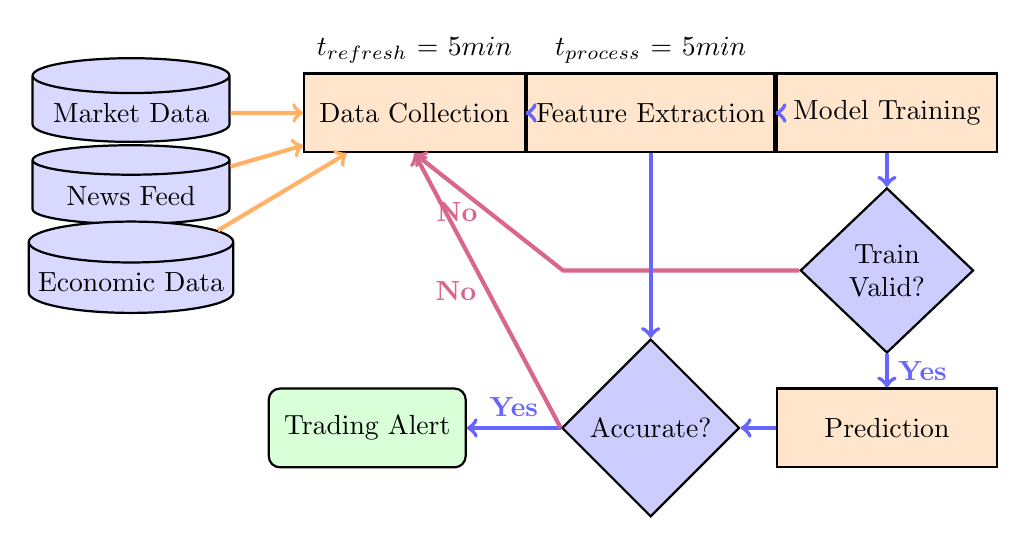
\begin{tikzpicture}[
        node distance=1.5cm,
        process/.style={rectangle, draw, fill=orange!20, minimum width=2.8cm, minimum height=1cm, thick},
        data/.style={cylinder, draw, fill=blue!15, shape border rotate=90, aspect=0.2, minimum width=2.5cm, minimum height=1cm, thick},
        decision/.style={diamond, draw, fill=blue!20, minimum width=2.2cm, minimum height=1.2cm, align=center, thick},
        action/.style={rectangle, draw, rounded corners, fill=green!15, minimum width=2.5cm, minimum height=1cm, thick},
        arrow/.style={->, line width=1.5pt, blue!60}
    ]
        % Data Sources
        \node[data] (market) at (-3.6,2) {Market Data};
        \node[data] (news) at (-3.6,0.95) {News Feed};
        \node[data] (econ) at (-3.6,-.15) {Economic Data};
        
        % Processing Nodes horizontal flow
        \node[process] (collect) at (0,2) {Data Collection};
        \node[process] (feature) at (3,2) {Feature Extraction};
        \node[process] (train) at (6,2) {Model Training};
        
        % Time labels above boxes
        \node[text width=2.8cm, align=center] at (0,2.8) {$t_{refresh}=5min$};
        \node[text width=2.8cm, align=center] at (3,2.8) {$t_{process}=5min$};
        
        % Validation and Prediction vertical flow
        \node[decision] (trainval) at (6,0.0) {Train\\ Valid?};
        \node[process] (predict) at (6,-2.0) {Prediction};
        
        % Alert and Trade
        \node[decision] (alert) at (3,-2.0) {Accurate?};
        \node[action] (trade) at (-0.6,-2.0) {Trading Alert};
        
        % Dependencies
        \draw[arrow, orange!60] (market) -- (collect);
        \draw[arrow, orange!60] (news) -- (collect);
        \draw[arrow, orange!60] (econ) -- (collect);
        \draw[arrow] (collect) -- (feature);
        \draw[arrow] (feature) -- (train);
        \draw[arrow] (train) -- (trainval);
        
        % Validation flows
        \draw[arrow] (trainval) -- node[right] {\textbf{Yes}} (predict);
        \draw[arrow, purple!60] (trainval.west) -- ++(-3,0) -- node[left] {\textbf{No}} (collect.south);
        
        % Real-time Flows
        \draw[arrow] (predict) -- (alert);
        \draw[arrow, blue!60] (feature) -- (alert);
        \draw[arrow] (alert) -- node[above] {\textbf{Yes}} (trade);
        \draw[arrow, purple!60] (alert.west) -- node[left] {\textbf{No}} (collect.south);
        
    \end{tikzpicture}
    \caption{Stock Market Prediction Workflow with Validation Loops. Two decision points validate: 1) model accuracy on testing data, and 2) real-time prediction accuracy for trading notifications.}
    \label{fig:P11workflow}
%    \vspace{.1in}
\end{figure*}


\noindent \textbf{Problem Specification:}

\noindent \underline{\textit{Setup:}}
\begin{itemize}[leftmargin=1.2em, topsep=-.0em, parsep=-.0em, label=*]
   \item \textit{Objective:} Predict a portfolio of stock prices for time \(\tau\), enabling actionable insights for risk management, investment decisions, and automated trading.
   \item \textit{Historical Data:}
   \begin{itemize}[leftmargin=1em, topsep=-.1em, parsep=-.1em]
       \item Training period: 2010--2020.
       \item Validation period: 2021--2023.
       \item Real-time data feed required during operation.
   \end{itemize}
   \item \textit{Data Sources:} Yahoo Finance, SEC EDGAR, news feeds, macroeconomic indicators.
   \item \textit{Required Features:}
   \begin{itemize}[leftmargin=1em, topsep=-.1em, parsep=-.1em]
       \item \textit{Technical Indicators:} MA, MACD, RSI, Bollinger Bands.
       \item \textit{Market Context:} Sector indices, competitor stock performance, correlation metrics.
       \item \textit{External Events:} Economic reports, policy changes, earnings announcements.
       \item \textit{Sentiment Analysis:} Real-time news, social media, financial disclosures.
   \end{itemize}
\end{itemize}

\noindent \underline{\textit{Constraints:}}
\begin{itemize}[leftmargin=1.5em, topsep=-.15em, parsep=-.15em, label=*]
   \item \textit{Processing latency:} Under 5 minutes for real-time predictions.
   \item \textit{Prediction confidence interval:} 95\% confidence bounds required.
   \item \textit{Model Dependencies:} 
   \begin{itemize}[leftmargin=1em, topsep=-.1em, parsep=-.1em]
       \item Data collection before feature extraction.
       \item Feature extraction before model training.
       \item Model training before prediction generation.
   \end{itemize}
   \item \textit{Performance Requirements:}
   \begin{itemize}[leftmargin=1em, topsep=-.1em, parsep=-.1em]
       \item Mean Absolute Percentage Error (MAPE) $<$ 5\% on validation.
       \item False alert rate $<$ 1\%.
       \item System uptime $>$ 99.9\% during market hours.
   \end{itemize}
\end{itemize}

\noindent \underline{\textit{State Space:}}
\begin{itemize}[leftmargin=1.5em, topsep=-.1em, parsep=-.1em, label=*]
    \item \textit{Processing Nodes ($V$):}
    \begin{itemize}[leftmargin=1em, topsep=-.1em, parsep=-.1em]
        \item Data Nodes: DC (data collection), FE (feature extraction).
        \item Model Nodes: MT (model training), PG (prediction generation).
        \item Integration Nodes: IG (integration), AG (alert generation).
    \end{itemize}
    \item \textit{Dependencies ($E$):}
    \begin{itemize}[leftmargin=1em, topsep=-.1em, parsep=-.1em]
        \item Pipeline: $DC \rightarrow FE \rightarrow MT \rightarrow PG \rightarrow AG$.
        \item Feedback: $AG \rightarrow DC$ for adaptive updates.
        \item External: Market events affect all nodes.
    \end{itemize}
\end{itemize}

\noindent \underline{\textit{Market Regime Adaptation:}}
\begin{itemize}[leftmargin=1.5em, topsep=-.1em, parsep=-.1em, label=*]
   \item Detect shifts in volatility, liquidity, and trend strength.
   \item Adjust prediction models based on regime detection.
   \item Implement fallback strategies for extreme market shifts.
\end{itemize}

\noindent \underline{\textit{Adaptive Refresh Rates:}}
\begin{itemize}[leftmargin=1.5em, topsep=-.1em, parsep=-.1em, label=*]
   \item \(t_{\text{Drefresh}}\) (data collection) adjusts based on market volatility.
   \item \(t_{\text{Nrefresh}}\) (news updates) increases during high-impact events.
\end{itemize}

\noindent \underline{\textit{Decision Module:}}
\begin{itemize}[leftmargin=1.5em, topsep=-.1em, parsep=-.1em, label=*]
   \item \textit{Trading Strategy:} Buy/sell signals, stop losses, risk thresholds.
   \item \textit{Risk Assessment:} Hedging, diversification, leverage constraints.
   \item \textit{Dynamic Adjustment:} Rebalancing frequency, asset weighting, market response.
\end{itemize}

\noindent \underline{\textit{Backtesting and Iterative Validation:}}
\begin{itemize}[leftmargin=1.5em, topsep=-.1em, parsep=-.1em, label=*]
   \item Run models on historical data to evaluate predictive accuracy.
   \item Compare performance on different market regimes/conditions.
   \item Adjust hyperparameters based on validation results.
\end{itemize}

\begin{table}[th!]
\centering
\caption{Stock Market Prediction Problem Framework}
%\vspace{-.1in}
\begin{small}
\renewcommand{\arraystretch}{1.1}
\fbox{
\begin{minipage}{0.45\textwidth}
\textbf{Network Structure:} $G=(V,E)$ where $V$ represents processing nodes and $E$ represents data flows

\textbf{Processing Nodes ($V$):}
\begin{itemize}[leftmargin=1em, topsep=-.1pt, itemsep=-.1pt, label=-]
\item Data nodes: DC (data collection), FE (feature extraction)
\item Model nodes: MT (model training), PG (prediction generation)
\item Integration nodes: IG (integration), AG (alert generation)
\end{itemize}

\textbf{Dependencies ($E$):}
\begin{itemize}[leftmargin=1em, topsep=-.1pt, itemsep=-.1pt, label=-]
\item Technical Analysis: $DC \rightarrow FE \rightarrow MT$
\item Market Context: External events affect all nodes
\item Model Chain: $MT \rightarrow PG \rightarrow AG$
\item Feedback Loop: $AG \rightarrow DC$ for adaptive updates
\end{itemize}

\textbf{Data Requirements:}
\begin{itemize}[leftmargin=1em, topsep=-.1pt, itemsep=-.1pt, label=-]
\item Historical: Training (2010--2020), Validation (2021--2023)
\item Technical Indicators: MA, BB, MACD, RSI, ATR, OBV
\item Price Data: OHLCV with adjustments
\item External: Policy, economic indices, news sentiment
\end{itemize}

\textbf{System Parameters:}
\[
\begin{aligned}
t_{refresh} &= 5 \text{ min}, \text{conf}_{interval} = 95\% \\
\text{MAPE} &< 5\%, \text{uptime} = 99.9\%
\end{aligned}
\]

\textbf{Workflow Stages:}
\begin{itemize}[leftmargin=1em, topsep=-.1pt, itemsep=-.1pt, label=-]
\item Stage 1: Data Collection \& Feature Extraction
\item Stage 2: Model Training \& Validation
\item Stage 3: Prediction Generation
\item Stage 4: Alert \& Decision Support
\item Stage 5: Iterative Refinement
\end{itemize}

\textbf{Dynamic Adaptations:}
\begin{itemize}[leftmargin=1em, topsep=-.1pt, itemsep=-.1pt, label=-]
\item Market regime shifts trigger model updates
\item News events modify prediction weights
\item Volatility affects refresh rates
\item Anomalies initiate retraining cycles
\end{itemize}

\textbf{Performance Metrics:}
\begin{itemize}[leftmargin=1em, topsep=-.1pt, itemsep=-.1pt, label=-]
\item Prediction accuracy (RMSE, MAPE)
\item System responsiveness (latency)
\item Alert precision (false positive rate)
\item Model adaptability (regime changes)
\end{itemize}
\end{minipage}
}
\end{small}
\label{tab:StockPrediction}
\end{table}


\begin{comment}
\begin{table}[thb]
\centering
\caption{Stock Market Prediction Problem}
\label{tab:StockPrediction}
\vspace{-.1in}
\begin{small}
\renewcommand{\arraystretch}{1.1}
\fbox{
\begin{minipage}{0.45\textwidth}

\textbf{The Problems}

\textbf{1) Stock Price Prediction:} Forecast future stock prices (e.g., predicting Apple’s stock on a future date) using historical market data.

\textbf{2) Complex Market Dynamics:} The system must account for influences such as technical indicators, historical price patterns, and external events (policy announcements, CPI, natural disasters, geopolitical conflicts).

\textbf{3) Decision Making Under Uncertainty:} Supports what-if analyses and real-time alerts for decision-makers to respond quickly to unexpected events.

\textbf{The State Space}

\textbf{1) Who:} Companies or stocks (e.g., Apple) and related market players (competitors, sector peers).

\textbf{2) What:}
\begin{itemize}[leftmargin=1em, topsep=-.1pt, itemsep=-.1pt, label=-]
\item Technical indicators: MA, BB, MACD, RSI, ATR, OBV, lagged closing prices.
\item Traditional price data: Open, high, low, close, adjusted close, trading volumes.
\item Self-defined features: News sentiment, policy announcements.
\end{itemize}

\textbf{3) When:}
\begin{itemize}[leftmargin=1em, topsep=-.1pt, itemsep=-.1pt, label=-]
\item Historical Data: Training (2010–2020), validation (2021–2023).
\item Future Forecasting: Target date (e.g., 2026-02-01).
\end{itemize}

\textbf{4) Where:} Market context including policy changes, economic reports (CPI), and geopolitical events.

\textbf{Interdependencies}

\textbf{1) Market Patterns and Correlations:} Identify how movements in one sector or competitor’s stock affect another.

\textbf{2) External Influences:} Policy announcements, economic reports, and disruptions (earthquakes, geopolitical crises) create cascading market effects.

\textbf{3) Integration of Data Types:} Combine numerical indicators, historical patterns, and qualitative information (news sentiment, human prompts) for a holistic market view.

\textbf{Proposed Workflow for Decision Making}

\textbf{1) Data Collection \& Feature Extraction:}
\begin{itemize}[leftmargin=1em, topsep=-.1pt, itemsep=-.1pt, label=-]
\item Gather historical market data (prices, volumes, technical indicators) from sources like Yahoo Finance and SEC EDGAR.
\item Integrate external data such as policy announcements and economic indices.
\end{itemize}

\textbf{2) Model Training \& Prediction:}
\begin{itemize}[leftmargin=1em, topsep=-.1pt, itemsep=-.1pt, label=-]
\item Use predictive models (Support Vector Regression, XGBoost, LSTM) to learn feature-stock price relationships.
\item Evaluate models using RMSE and validation datasets.
\end{itemize}

\textbf{3) Integration \& Optimization:}
\begin{itemize}[leftmargin=1em, topsep=-.1pt, itemsep=-.1pt, label=-]
\item Combine multiple features and models (meta-planning) to optimize predictions.
\item Adjust hyperparameters, refine features iteratively.
\end{itemize}

\textbf{4) Decision Support \& Real-Time Alerts:}
\begin{itemize}[leftmargin=1em, topsep=-.1pt, itemsep=-.1pt, label=-]
\item Perform what-if analyses to predict event impacts (e.g., policy changes, natural disasters).
\item Set up alerts for sudden market changes.
\end{itemize}

\textbf{5) Iterative Validation \& Refinement:} Continuously validate predictions with new data, refining models based on feedback.

\end{minipage}
}
\end{small}
\end{table}
\begin{table}[thb]
\centering
\caption{Meta Plan based on Stock Prediction Specification}
\label{tab:MetaPlanner}
\vspace{-.1in}
\begin{small}
\renewcommand{\arraystretch}{1.1}
\fbox{
\begin{minipage}{0.45\textwidth}


\textbf{Step 1: Define Objectives} 

\begin{equation} 
{\mathcal{O} = \{ \text{Forecast future stock prices}, \text{Integrate external influences}, 
\\
\text{Support decision making with real-time alerts} \}}
\end{equation}

\textbf{Step 2: Identify Explicit Constraints}
\begin{equation}
\mathcal{C}_{\mathcal{E}} = \{ \text{Use historical data from 2010 to 2020}, \text{Consider external events}, \\
\text{Ensure compliance with market regulations} \}
\end{equation}

\textbf{Step 3: Identify Implicit Constraints}
\begin{equation}
\mathcal{C}_{\text{I}} = \{ \text{Market trends influence stock prices}, \text{Technical indicators \\
provide insights} \}
\end{equation}

\textbf{Step 4: Define the Agent Pool}
\begin{equation}
A = \{ \text{Support Vector Regression}, \text{XGBoost}, \text{LSTM}, \text{Random Forest}, \text{\\
Expert Systems} \}
\end{equation}

\textbf{Step 5: Define Performance Metrics}
\begin{equation}
\mathcal{M} = \{ \text{Mean Absolute Error (MAE)}, \text{Root Mean Squared Error (RMSE)}, \\
\text{R-squared value} \}
\end{equation}

\textbf{Step 6: Construct the Workflow Network}
\begin{itemize}
\item \textbf{Roles:} Data collection, feature extraction, model training, prediction, integration, optimization, decision support.
\item \textbf{Dependencies:} Data must be collected before feature extraction, and so on.
\end{itemize}
\begin{equation}
\mathcal{N} = \{ \text{Data Collection}, \text{Feature Extraction}, \text{Model Training}, \text{Prediction}, \\ 
\text{Integration}, \text{Decision Support}, \text{Validation} \}
\end{equation}
\begin{equation}
\mathcal{E} = \{ \text{Collection} \rightarrow \text{Feature Extraction}, \text{Feature Extraction} \rightarrow \text{Model \\ Training}, \text{Model Training} \rightarrow \text{Prediction}, \text{Prediction} \rightarrow \text{Integration}, \text{Integration} \rightarrow \text{Decision Support}, \text{Decision Support} \rightarrow \text{Validation} \}
\end{equation}

\textbf{Step 7: Assign Agents to Nodes and Edges}
\begin{equation}
A_{n}^{*} = \{ \text{Web Scraper}, \text{Data Cleaning Algorithm}, \text{Support Vector \\ Regression}, \text{XGBoost}, \text{LSTM} \}
\end{equation}
\begin{equation}
A_{e}^{*} = \{ \text{Dependency Management Algorithm} \}
\end{equation}

\textbf{Step 8: Iterative Refinement}
\begin{itemize}
\item Evaluate workflow using performance metrics.
\item Update role-agent mappings based on performance feedback.
\item Verify dependencies for correctness.
\end{itemize}

\textbf{Final Workflow Representation}
\begin{equation}
\mathbf{W}^{*} = (\mathcal{N}, \mathcal{E})
\end{equation}

\end{minipage}
}
\end{small}
\end{table}

\end{comment}



\subsection{Execution Example: Urban Ride Sharing }

For a benchmark suite, we encourage users to
devise novel methodologies to solve the problems. However, for this illustrative example of Urban Ride Sharing (URS) (P3), we employ a customized specification language that extends PDDL (Planning Domain Definition Language) and workflow networks to support:

\begin{itemize}[leftmargin=1.0em, topsep=-.0em, parsep=-.0em, label=-]
    \item Dynamic constraints and real-time updates.
    \item Integration with streaming data sources.
    \item Explicit representation of uncertainty.
    \item Temporal and spatial dependencies.
\end{itemize}

The solver, whether manual or automatic, approaches the planning problem in three steps:
\begin{enumerate}[leftmargin=1.0em, topsep=-.0em, parsep=-.0em, label=\arabic*.]
    \item Convert the problem statement into a formal specification:
    \begin{itemize}[leftmargin=1em, topsep=-0em, parsep=-0em, label=-]
        \item Key objectives and constraints.
        \item Required resources and their capabilities.
        \item Performance metrics and success criteria.
        \item Temporal and spatial dependencies.
    \end{itemize}
    
    \item Transform the specification into a workflow graph:
    \begin{itemize}[leftmargin=1em, topsep=-0em, parsep=-0em, label=-]
        \item Nodes represent processing stages, decision points, or actions.
        \item Edges capture dependencies, data flow, and execution sequence.
        \item Agents are assigned to both nodes and edges.
        \item Concrete parameters and thresholds are specified.
    \end{itemize}
    
    \item Select and apply solving algorithms:
    \begin{itemize}[leftmargin=1em, topsep=0em, parsep=0em, label=-]
        \item Test multiple solution approaches (e.g., dynamic programming, Monte Carlo).
        \item Evaluate solutions against specified metrics.
        \item Select and validate the best-performing solution.
        \item Present results with performance analyses.
    \end{itemize}
\end{enumerate}

We walk through these three steps to solve the URS problem.

\subsubsection{URS Problem Specification}Already presented in Table~\ref{tab:appURS}.

\subsubsection{URS Workflow}

Figure~\ref{fig:URS-DirectedGraph} shows
the workflow representation of the URS problem.

\begin{figure}[th!]
%\vspace{-.1in}
    \centering
    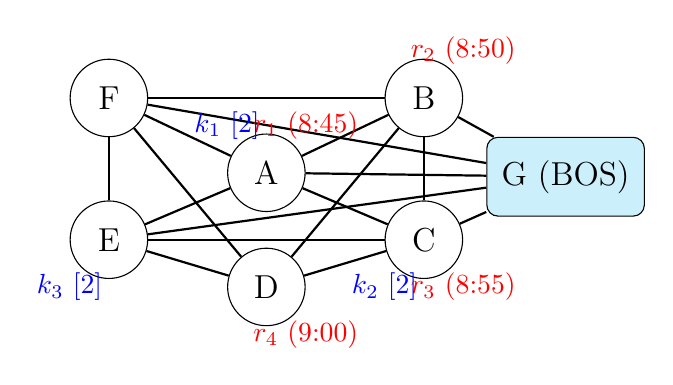
\begin{tikzpicture}[
        location/.style={
            circle,
            draw=black,
            fill=white!20,
            minimum size=0.8cm,
            text centered,
            font=\large
        },
        airport/.style={
            rectangle,
            rounded corners,
            draw=black,
            fill=cyan!20,
            minimum width=2.0cm,
            minimum height=1.0cm,
            text centered,
            font=\large
        },
        passenger/.style={
            font=\normalsize\color{red}
        },
        vehicle/.style={
            font=\normalsize\color{blue}
        },
        urban_path/.style={thick},
        airport_path/.style={thick}
    ]
        % Title
        %\node[draw=none] at (0,4) {\Large Urban Ride Sharing Network};
        
        % Urban locations
    \node[location, fill=white, draw, inner sep=2pt, minimum size=28pt] (A) at (0,1.05) {A};
    \node[location, fill=white, draw, inner sep=2pt, minimum size=28pt] (B) at (2.0,2) {B};
    \node[location, fill=white, draw, inner sep=2pt, minimum size=28pt] (C) at (2.0,0.2) {C};
    \node[location, fill=white, draw, inner sep=2pt, minimum size=28pt] (D) at (0,-0.4) {D};
    \node[location, fill=white, draw, inner sep=2pt, minimum size=28pt] (E) at (-2.0,0.2) {E};
    \node[location, fill=white, draw, inner sep=2pt, minimum size=28pt] (F) at (-2.0,2) {F};

        % Airport location
        \node[airport] (G) at (3.8,1) {G (BOS)};
        
        % Urban routes with time only
        \foreach \from/\to in {A/B, B/C, C/D, D/E, E/F, F/A, A/C, B/D, C/E, D/F, E/A, F/B}
            \draw[urban_path] (\from) -- (\to) 
            node[midway,fill=none] {};
            
        % Airport routes with time only
        \draw[airport_path] (A) -- (G) node[pos=0.72,sloped,above,fill=none] {};
        \draw[airport_path] (B) -- (G) node[pos=0.50,sloped,above,fill=none] {};
        \draw[airport_path] (C) -- (G) node[pos=0.50,sloped,above,fill=none] {};
%        \draw[airport_path] (D) -- (G) node[pos=0.72,sloped,above,fill=none] {};
        \draw[airport_path] (E) -- (G) node[pos=0.78,sloped,above,fill=none] {};
        \draw[airport_path] (F) -- (G) node[pos=0.78,sloped,above,fill=none] {};
        
        % Passengers with arrival times
        \node[passenger] at ($(A)+(0.5,0.6)$) {$r_1$ (8:45)};
        \node[passenger] at ($(B)+(0.5,0.6)$) {$r_2$ (8:50)};
        \node[passenger] at ($(C)+(0.5,-0.6)$) {$r_3$ (8:55)};
        \node[passenger] at ($(D)+(0.5,-0.6)$) {$r_4$ (9:00)};
        
        % Vehicles with capacities
        \node[vehicle] at ($(A)+(-0.5,0.6)$) {$k_1$ [2]};
        \node[vehicle] at ($(C)+(-0.5,-0.6)$) {$k_2$ [2]};
        \node[vehicle] at ($(E)+(-0.5,-0.6)$) {$k_3$ [2]};
        
    \end{tikzpicture}
    %\vspace{-.15in}
    \caption{Consider a network $G=(V,E)$ with urban travel times $\tau_{ij}=10$ minutes and airport routes $\tau_{iG}=\{19,\ldots,22\}$ minutes. Schedule three vehicles $k_i$ (capacity $c_k=2$) to deliver four passengers $r_i$ to airport during $[8:45,9:00]$.}\Description{URS}
    %\vspace{-.1in}
    \label{fig:URS-DirectedGraph}
\end{figure}
%\vspace{-.2in}


\subsubsection{URS Results}

Figure~\ref{fig:ALASmonte-carlo} presents an optimal solution with a total travel distance of 87 km, outperforming both GPT-4o-Task and DeepSeek R1 (Figure~\ref{fig:GPTDS-schedule}), which require 123 km. This represents a significant improvement of 41.37\%.

\paragraph{Extended Materials}

We also used LangGraph to implement both \textbf{P3} and \textbf{P4}, as presented in \textbf{Appendix}~\ref{app:p3p4}. Furthermore, we provide a solution to \textbf{P11} for the prediction of the stock value. These sample implementations validate the completeness of the problem statements in this benchmark.

\begin{figure}[ht!]
%\vspace{-.1in}
    \centering
    \begin{tikzpicture}[
        location/.style={
            circle,
            draw=black,
            fill=white,
            minimum size=1.0cm,
            text centered,
            font=\normalsize
        },
        airport/.style={
            rectangle,
            rounded corners,
            draw=black,
            fill=cyan!20,
            minimum width=2.0cm,
            minimum height=1.0cm,
            text centered,
            font=\normalsize
        },
        passenger/.style={
            font=\small\color{red}
        },
        path_k1/.style={
            thick,
            blue,
            ->,
            >=stealth
        },
        path_k2/.style={
            thick,
            orange,
            ->,
            >=stealth
        },
        vehicle/.style={
            draw,
            fill=white,
            minimum width=0.8cm,
            minimum height=0.4cm,
            rounded corners=1pt
        }
    ]
         % Vehicle k1 at A
        \node[blue] at (-1,1.5) {\Huge\faTaxi};
        \node[blue] at (-1,2.0) {k1};

        % Urban locations
        \node[location] (A) at (0,1.5) {A};
        \node[location] (B) at (2.1,1.5) {B};
        \node[location] (C) at (0,0) {C};
        \node[location] (D) at (2.1,0) {D};
        
        % Vehicle k2 at C
        \node[orange] at (-1,0) {\Huge\faTaxi};
        \node[orange] at (-1,0.5) {k2};
        
        % Airport location with arrival times
        \node[airport] (G) at (5,.75) {G (BOS)};
        
        % k1 path: A -> B -> G
        \draw[path_k1] (A) -- (B) node[midway,above,sloped,fill=none,font=\footnotesize] {8:00-8:10};
        \draw[path_k1] (B) -- (G) node[midway,above,sloped,fill=none,font=\footnotesize] {8:10-8:30};
        
        % k2 path: C -> D -> G
        \draw[path_k2] (C) -- (D) node[midway,below,fill=none,font=\footnotesize] {8:00-8:10};
        \draw[path_k2] (D) -- (G) node[midway,below,sloped,fill=none,font=\footnotesize] {8:10-8:30};
        
        % Passengers with arrival times
        \node[passenger] at ($(A)+(0.3,0.7)$) {$r_1$ (8:45)};
        \node[passenger] at ($(B)+(0.3,0.7)$) {$r_2$ (8:50)};
        \node[passenger] at ($(C)+(0.3,0.7)$) {$r_3$ (8:55)};
        \node[passenger] at ($(D)+(0.3,0.7)$) {$r_4$ (9:00)};
        
    \end{tikzpicture}
    %\vspace{-.1in}
    \caption{This solution routes showing optimal vehicle assignments. Vehicle k1 (blue) starts at A and collects passengers r1 and r2, while k2 (orange) starts at C and serves r3 and r4. Both vehicles arrive at BOS at 8:30, meeting all passenger arrival deadlines. Total distance traveled = 87 km ({\color{red}Optimal}).}\Description{This figure illustrates the optimal vehicle assignments for the ALAS solution routes, showing vehicles k1 and k2 serving passengers and meeting deadlines.}
    \label{fig:ALASmonte-carlo}
    %\vspace{-.1in}
\end{figure}
%\vspace{-.15in}
\begin{figure}[ht!]
%\vspace{-.1in}
    \centering
    \begin{tikzpicture}[
        location/.style={
            circle,
            draw=black,
            fill=white,
            minimum size=1.0cm,
            text centered,
            font=\normalsize
        },
        airport/.style={
            rectangle,
            rounded corners,
            draw=black,
            fill=cyan!20,
            minimum width=2cm,
            minimum height=1cm,
            text centered,
            font=\normalsize
        },
        passenger/.style={
            font=\small\color{red}
        },
        path_k1/.style={
            thick,
            blue,
            ->,
            >=stealth
        },
        path_k2/.style={
            thick,
            orange,
            ->,
            >=stealth
        },
        path_k3/.style={
            thick,
            green!50!black,
            ->,
            >=stealth
        },
        vehicle/.style={
            draw,
            fill=white,
            minimum width=0.8cm,
            minimum height=0.4cm,
            rounded corners=1pt
        }
    ]
        % Vehicle k1 icon at A

        % Replace vehicle nodes with faTaxi icons

        % Vehicle k1 at A
        \node[blue] at (-1,1.5) {\Huge\faTaxi};
        \node[blue] at (-1,2.0) {k1};


        % Urban locations in more compact arrangement
        \node[location] (A) at (0,1.6) {A};
        \node[location] (B) at (2.1,1.6) {B};
        \node[location] (C) at (3.8,0) {C};
        \node[location] (E) at (0,0) {E};
        \node[location] (D) at (2.0,0) {D};
        
        % Vehicle k2 at C
        \node[orange] at (4.8,0) {\Huge\faTaxi};
        \node[orange] at (4.8,0.5) {k2};


        % Vehicle k3 at E
        \node[green!50!black] at (-1,0) {\Huge\faTaxi};
        \node[green!50!black] at (-1,0.5) {k3};
        
        % Airport location moved higher
        \node[airport] (G) at (5.0,1.6) {G (BOS)};
        
        % k1 path: A -> B -> G
        \draw[path_k1] (A) -- (B) node[midway,above,font=\footnotesize] {7:40-7:50};
        \draw[path_k1] (B) -- (G) node[midway,above,fill=none,font=\footnotesize] {7:50-8:10};
        
        % k2 path: C -> G
        \draw[path_k2] (C) -- (G) node[pos=0.58,sloped,below,fill=none,font=\footnotesize] {7:55-8:17};

        % k3 path: E -> D
        \draw[path_k3] (E) -- (D) node[midway,sloped,above,fill=none,font=\footnotesize] {7:50-8:00};
        
        
        % k3 path: E -> G
        \draw[path_k3] (D) -- (G) node[pos=0.66,sloped,above,fill=none,font=\footnotesize] {8:00-8:19};
        
        % Passengers with arrival times
        \node[passenger] at ($(A)+(0.3,0.7)$) {$r_1$ (8:45)};
        \node[passenger] at ($(B)+(0.3,0.7)$) {$r_2$ (8:50)};
        \node[passenger, fill=none, inner sep=2pt] at ($(C)+(0.0,0.65)$) {$r_3$};


        %\node[passenger] at ($(C)+(0.3,0.70)$) {$r_3$ (8:55)};
        \node[passenger] at ($(D)+(0.3,0.7)$) {$r_4$ (9:00)};
        
    \end{tikzpicture}
    %\vspace{-.1in}
    \caption{GPT-4o-Task and DeepSeek R1 both schedule three routes. Vehicle k1 picks up r1 from A at 7:40, then r2 from B at 7:50. Vehicle k2 picks up r3 from C at 7:55. Vehicle k3 must first drive from E to D to pick up r4 at 8:00. All meet deadlines. Total travel distance = 123 km.}\Description{Infeasible Schedule}
    \label{fig:GPTDS-schedule}
    %\vspace{-.1in}
\end{figure}
%\vspace{-.1in}

Software development is increasingly conceived as a collaboration activity between developers and AIs. Indeed, IDEs already implement features to enable interactive development, with AI suggesting implementations that are reused by developers.

Although multiple studies show this interaction can be successful, there is still limited understanding of how the models must be configured and used in the context of code generation tasks. This study addresses this gap, systematically investigating the impact of several key parameters, including the repeated submission of a prompt to accommodate for the non-deterministic nature of the models.

Our study reveals several key findings about the usage of ChatGPT. In particular, we discovered how creativity, although up to a limited extent, is useful to increase the range of methods whose code can be generated correctly. A major role is played by parameter top-p, which is commonly underrated, and instead has a major impact on the correctness of the results, with lower values producing better results. Finally, prompts should be submitted multiple times, with $5$ repetitions combined with a temperature of $1.2$ resulting in an effective configuration in our experiments.  

Future work concerns two main research directions. One is about replicating this experiment with other AI assistants, to validate our findings in multiple contexts. The second research direction concerns finding strategies to deal with the need to submit the same prompt multiple times to obtain a useful result, and thus developing approaches able to select or merge multiple responses automatically. 
%\input{BenchmarkInstructions}

\bibliographystyle{ACM-Reference-Format}
\bibliography{BenchmarkReference, EdwardChang}


%%
%% If your work has an appendix, this is the place to put it.
\appendix

\section*{Appendices}

In these Appendices, we provide sample implementations of selected problems, illustrating that each problem specification is implementable and can produce feasible solutions. This serves as a verification of completeness for the problem definitions. We encourage readers to review the code and use it as a reference for designing improved solutions to these challenges.

The three problems selected are \textbf{P3}, \textbf{P4}, and \textbf{P11}, representing sequential planning, reactive planning, and the most complex planning scenario, respectively.

\section{P3 \& P4: Urban Ride Sharing Sample Implementation}
\label{app:p3p4}

This appendix presents an implementation of \textbf{P3} and \textbf{P4}: Urban Ride Sharing without and with interrupts, using LangGraph~\cite{langgraph2024}.

\subsection{Agentic Workflow Formulation}

In this first stage, we define agents to manage the nodes of the workflow, including data collection, route planning, vehicle dispatch, traffic adjustment, monitoring and alert, and logging agents. At the end, we use the \texttt{>>} syntax to specify dependencies among agents. The transition from problem specifications to workflow formulation is handled automatically by MACI\,\cite{chang2025MACI} in LangGraph.

\begin{lstlisting}[style=PythonStyle, caption=Collaborative Agents and Prompts, label=lst:agent_pipelinep3p4]
    # ---- Data Collection Agent ---- #
    DC_Agent = Agent(
        name=``Data Collection Agent'',
        backstory=``You collect basic traffic data, road closure updates, and estimated travel times between locations in Bay Area suburb.'',
        task_description=``Retrieve traffic conditions, road closures, and estimated travel durations for all routes involved in passenger transport.'',
        task_expected_output=``Structured travel time data, including:
        1) CityMap: A graph G = (V, E), where the locations V and roads E have distances and travel times.
        2) Ride Requests: A set of requests R, each defined by: PassengerID, pickup/drop-off locations, and time windows.
        3) Vehicles: A set of available vehicles K, each with location, battery/fuel level, passenger capacity, and speed.'')
        
    # ---- Route Planning Agent ---- #
    RP_Agent = Agent(
        name=``Route Planning Agent'',
        backstory=``You determine optimal routes for vehicles to minimize total travel time while ensuring all passengers arrive on time.'',
        task_description=``Use traffic data and constraints to compute the best routes for each vehicle, ensuring on-time airport arrivals.'',
        task_expected_output=``Optimized vehicle assignments and travel routes.'')
    
    # ---- Vehicle Dispatch Agent ---- #
    VD_Agent = Agent(
        name=``Vehicle Dispatch Agent'',
        backstory=``You assign passengers to vehicles and ensure each vehicle follows the optimal planned route,'',
        
        task_description=``Assign passengers to vehicles based on capacity constraints and route efficiency,''
        
        task_expected_output=``Vehicle assignment list and dispatch schedule.'')
    
    # ---- Traffic Adjustment Agent (e.g. disruptions, special cases)---- #
    TA_Agent = Agent(
        name=``Traffic Adjustment Agent'',
        backstory=``You monitor live traffic updates and adjust vehicle routes dynamically in case of delays in Bay Area suburb.'',
        task_description=``Recompute routes in real time when disruptions occur (traffic, road closures), ensuring minimal delays.'',
        task_expected_output=``Updated travel plans for affected vehicles.'')
    
    # ---- Monitoring & Alert Agent ---- #
    MA_Agent = Agent(
        name=``Monitoring & Alert Agent'',
        backstory=``You track vehicle movements and notify if there are risks of missing passenger deadlines in Bay Area suburb.'',
        task_description=``Send alerts for potential delays and recommend contingency plans.'',
        task_expected_output=``Timely notifications for alternative route adjustments or emergency responses.'')
    
    Writer_agent = Agent(
        name=``Writer Agent'',
        backstory=``You are a language model specialized in writing text into .json files'',
        task_description=``Write the json response into ./p3_output.json'',
        task_expected_output=``A .json file containing the given string,
        tools=write_str_to_txt'')

    # ---- Define Dependencies (With Disruption) ---- #
    DC_Agent >> RP_Agent >> VD_Agent >> TA_Agent >> MA_Agent >> Writer_agent

    # ---- Define Dependencies (Without Disruption) ---- #
    DC_Agent >> RP_Agent >> VD_Agent >> MA_Agent >> Writer_agent

\end{lstlisting}

\subsection{P3: Execute Meta Plan without Disruption}

Now that the meta-plan workflow has been constructed, the second step involves providing real data for workflow execution. The following code snippet illustrates how vehicle and passenger locations are specified, followed by the corresponding agent executions.

\begin{lstlisting}[style=JSONStyle, caption=Sample JSON Output from Agentic Workflow, label=lst:data_collectionp3p4]
==================================================
RUNNING AGENT: Data Collection Agent
==================================================
1) \textbf{CityMap: A graph G=(V,E)}
   - \textbf{Locations V:}
     - V1: Downtown
     - V2: Golden Gate Park
     - V3: Fisherman Wharf
     - V4: Union Square
     - V5: San Francisco Airport (SFO)

   - \textbf{Roads E with distances and travel times:}
     - E1: Downtown to Golden Gate Park, Distance: 5 miles, Travel Time: 20 minutes
     - E2: Golden Gate Park to Fisherman Wharf, Distance: 6 miles, Travel Time: 25 minutes
     - E3: Fisherman Wharf to Union Square, Distance: 2 miles, Travel Time: 10 minutes
     - E4: Union Square to SFO, Distance: 15 miles, Travel Time: 30 minutes
     - E5: Downtown to SFO, Distance: 13 miles, Travel Time: 35 minutes

2) \textbf{Ride Requests: A set of requests R}
   - Request 1:
     - PassengerID: P001
     - Pickup: Downtown
     - Drop-off: Union Square
     - Time Window: 9:00 AM - 9:30 AM
   - Request 2:
     - PassengerID: P002
     - Pickup: Golden Gate Park
     - Drop-off: SFO
     - Time Window: 10:00 AM - 11:00 AM
   - Request 3:
     - PassengerID: P003
     - Pickup: Fisherman Wharf
     - Drop-off: Downtown
     - Time Window: 1:00 PM - 1:30 PM

3) \textbf{Vehicles: A set of available vehicles K}
   - Vehicle 1:
     - Location: Downtown
     - Battery/Fuel Level: 80%
     - Passenger Capacity: 4
     - Speed: 30 mph
   - Vehicle 2:
     - Location: Union Square
     - Battery/Fuel Level: 60%
     - Passenger Capacity: 6
     - Speed: 25 mph
   - Vehicle 3:
     - Location: SFO
     - Battery/Fuel Level: 90%
     - Passenger Capacity: 3
     - Speed: 35 mph

This structured data provides an overview of the current traffic conditions, road closures, and estimated travel times for passenger transport in SF.

================================================== 
RUNNING AGENT: Route Planning Agent
==================================================
Optimized vehicle assignments and travel routes:

1) \textbf{Vehicle Assignments:}

   - Vehicle 1:
     - Assigned to Request 1
     - Route: Downtown (V1) -> Union Square (V4)
     - Estimated Travel Time: 20 minutes (E1 + E3)
     - Departure Time: 9:00 AM
     - Arrival Time: 9:20 AM

   - Vehicle 2:
     - Assigned to Request 2
     - Route: Union Square (V4) -> Golden Gate Park (V2) -> SFO (V5)
     - Estimated Travel Time: 55 minutes (E3 + E2 + E4)
     - Departure Time: 10:00 AM
     - Arrival Time: 10:55 AM

   - Vehicle 3:
     - Assigned to Request 3
     - Route: Fisherman Wharf (V3) -> Downtown (V1)
     - Estimated Travel Time: 10 minutes (E3)
     - Departure Time: 1:00 PM
     - Arrival Time: 1:10 PM

2) \textbf{Travel Routes:}

   - Request 1:
     - Vehicle 1 will pick up Passenger P001 at Downtown and drop off at Union Square.
     - Route: V1 -> V4

   - Request 2:
     - Vehicle 2 will pick up Passenger P002 at Golden Gate Park and drop off at SFO.
     - Route: V4 -> V2 -> V5

   - Request 3:
     - Vehicle 3 will pick up Passenger P003 at Fisherman Wharf and drop off at Downtown.

==================================================
RUNNING AGENT: Vehicle Dispatch Agent
==================================================
Vehicle Assignment List and Dispatch Schedule:

1) \textbf{Vehicle Assignments:}

   - Vehicle 1:
     - Assigned to Request 1
     - Passengers: P001
     - Route: Downtown (V1) -> Union Square (V4)
     - Estimated Travel Time: 20 minutes
     - Departure Time: ``9:00 AM''
     - Arrival Time: ``9:20 AM''

   - Vehicle 2:
     - Assigned to Request 2
     - Passengers: P002
     - Route: Union Square (V4) -> Golden Gate Park (V2) -> SFO (V5)
     - Estimated Travel Time: 55 minutes
     - Departure Time: ``10:00 AM''
     - Arrival Time: ``10:55 AM''

   - Vehicle 3:
     - Assigned to Request 3
     - Passengers: P003
     - Route: Fisherman Wharf (V3) -> Downtown (V1)
     - Estimated Travel Time: 10 minutes
     - Departure Time: ``1:00 PM''
     - Arrival Time: ``1:10 PM''

2) \textbf{Dispatch Schedule:}

   - 9:00 AM: Vehicle 1 departs from Downtown with Passenger P001.
   - 9:20 AM: Vehicle 1 arrives at Union Square.
   - 10:00 AM: Vehicle 2 departs from Union Square with Passenger P002.
   - 10:55 AM: Vehicle 2 arrives at SFO.
   - 1:00 PM: Vehicle 3 departs from Fisherman Wharf with Passenger P003.
   - 1:10 PM: Vehicle 3 arrives at Downtown.

These assignments and schedules ensure efficient use of vehicles and timely arrival of all passengers.

==================================================
RUNNING AGENT: Monitoring & Alert Agent
==================================================
\textbf{Alert Notification:}

1) Vehicle 1:
   - Current Status: On schedule.
   - Recommendation: No action needed as the vehicle is expected to arrive on time.

2) Vehicle 2:
   - Current Status: Potential delay risk due to high traffic expected around Golden Gate Park.
   - Recommendation: Consider adjusting the route to avoid traffic congestion. Possible alternative: Take the route via Sunset Blvd to bypass heavy traffic areas. Notify the passenger of the potential delay and the alternative route.

3) Vehicle 3:
   - Current Status: On schedule.
   - Recommendation: No action needed as the vehicle is expected to arrive on time.

\textbf{Contingency Plan:}

Emergency Response: If Vehicle 2 faces unexpected delays despite the alternative route, prepare a standby vehicle for immediate dispatch from a nearby location to ensure Passenger P002 reaches SFO on time.

==================================================
RUNNING AGENT: Writer Agent
==================================================
Thought: I need to write the given context string into a JSON file named ``./p3_output.json''.

Using Tool: write_str_to_txt
Tool call dict: {omitted}
Data successfully written to ``./p3_output.json''
Tool result: None
Observations: {0: None}
The context string has been successfully written into ``./p3_output.json'' as a JSON file.

\end{lstlisting}

\subsection{P4: Execute Meta Plan with Disruption}

This section depicts the execution of the meta-plan (workflow) under traffic disruption. In this scenario, the system dynamically identifies traffic delays and integrates real-time updates into the planning process. Each agent plays a crucial role: the data collection agent continuously monitors traffic conditions; the route planning agent adjusts travel routes based on congestion data; and the dispatch agent ensures that vehicle assignments are optimized despite delays. The workflow demonstrates how coordinated agent interventions, including dynamic rerouting and schedule adjustments, effectively mitigate the impact of heavy traffic, maintaining timely transportation, and enhancing overall operational efficiency.

\begin{lstlisting}[style=JSONStyle, caption=Sample JSON Output from Agent Pipeline, label=lst:disruptionp3p4]
==================================================
RUNNING AGENT: Traffic Adjustment Agent
==================================================
1) \textbf{Vehicle V1 (Passenger 101):}
   - \textbf{Current Disruption:} Heavy traffic reported on the route from Downtown SF to SF Airport.
   - \textbf{Updated Route:}
     - Start at Union Square
     - Travel to Downtown SF (2 miles, 15 minutes)
     - Detour via I-280 South instead of the usual route to SF Airport
     - Estimated travel time via detour: 30 minutes
   - \textbf{Total Updated Estimated Travel Time:} 45 minutes
   - \textbf{Revised Departure Time:} ``08:15'' to ensure timely arrival within the window.
   - \textbf{Special Instructions:} Maintain communication with the passenger about the updated route and expected arrival time.

2) \textbf{Vehicle V2 (Passenger 102):}
   - \textbf{Current Disruption:} Road closure near Fisherman Wharf due to an event.
   - \textbf{Updated Route:}
     - Start at Fisherman Wharf
     - Detour via Bay Street to Van Ness Avenue, then proceed to Golden Gate Bridge
     - Estimated travel time via detour: 15 minutes
   - \textbf{Total Updated Estimated Travel Time:} 15 minutes
   - \textbf{Revised Departure Time:} ``09:15'' to ensure timely arrival within the window.
   - \textbf{Special Instructions:} Ensure fuel levels are adequate for the detour and communicate any changes to the passenger.

\end{lstlisting}

%\begin{comment}

\documentclass{article}
\usepackage{listings}
\usepackage{xcolor}

% Define custom style for Python code
\lstdefinestyle{PythonStyle}{
    language=Python,
    basicstyle=\ttfamily\footnotesize,
    keywordstyle=\color{blue},
    commentstyle=\color{green},
    stringstyle=\color{red},
    breaklines=true,
    frame=single
}

% Define custom style for JSON
\lstdefinestyle{JSONStyle}{
    language=Java,
    basicstyle=\ttfamily\footnotesize,
    keywordstyle=\color{blue},
    stringstyle=\color{red},
    breaklines=true,
    frame=single
}

%\begin{document}
\end{comment}

\section{P5\&8: Wedding Logistics Problem Sample Implementation With and Without Update}

This appendix presents an implementation of the P5 and P8: Wedding Logistics Problem Without and With Disruption using LangGraph~\cite{langgraph2024}. 
\subsection{Prompt and Collaborative Agent Pipeline}

\begin{lstlisting}[style=PythonStyle, caption=Prompt and Collaborative Agent Pipeline, label=lst:agent_pipeline]
with Crew() as crew:
    # ---- Locations and Time Setup Agent ---- #
    LT_Agent = Agent(
        name="Locations and Time Setup Agent",
        backstory="You define locations, travel times, and guest arrival schedules.",
        task_description="Set up locations, travel times, and ensure accurate scheduling of arrivals.",
        task_expected_output="Structured location data and expected arrival times. Fourlocations:V ={B,G,T,W},where B isBostonAir- port, G is Gift shop, T is Tailor shop, and W is Wedding venue. B-G : 45, B-T : 30, B-W : 40, G-T : 20, G-W : 25, T-W : 15. - Alex:At B at11:00AMfromChicago(needaride) - Jamie:At B at12:30PMfromAtlanta(needaride) - Pat: At W at 12:00 PM driving from NYC (has 5-seater car)"
    )
    
    # ---- Task Setup Agent ---- #
    TS_Agent = Agent(
        name="Task Setup Agent",
        backstory="You manage the scheduling of required wedding tasks.",
        task_description="Schedule gift collection after 12:00 PM, clothes pickup before 2:00 PM, and ensure photo session at 3:00 PM.",
        task_expected_output="Optimized task schedule aligned with constraints."
    )

    # ---- Disruption Update Agent (With Disruption) ---- #
    DU_Agent = Agent(
        name="Disruption Update Agent",
        backstory="You monitor road closures and dynamically reroute transportation as needed.",
        task_description="Identify any road closures or unexpected disruptions and adjust travel plans accordingly.",
        task_expected_output="In case there is road closures of B to G, and dynamically reroute transportation. Updated task schedule, ensuring minimal delays and timely arrivals with new updates."
    )
    
    # ---- Resource Management Agent ---- #
    RM_Agent = Agent(
        name="Resource Management Agent",
        backstory="You allocate available transport resources efficiently.",
        task_description="Coordinate 5 vehicle usage and Local friend Chris(5-seater)available, for guest transportation and task fulfillment.",
        task_expected_output="Optimized 5 vehicle allocation and friend welcome ensuring timely arrivals. - Onecar(5-seater)withPat,availableafterheisBoston - LocalfriendChris(5-seater)availableafter1:30PM at W"
    )
    
    # ---- Constraint Validation Agent ---- #
    CV_Agent = Agent(
        name="Constraint Validation Agent",
        backstory="You verify all scheduling constraints to ensure smooth execution.",
        task_description="Ensure all tasks are completed within operating hours and vehicle constraints are met.",
        task_expected_output="Validated schedule with no conflicts. All tasks must complete before 3:00 PM photo time - Gift store opens at 12:00 PM - Tailor closes at 2:00 PM - Two cars must accommodate all transport needs"
    )

    # ---- Supervisor Agent ---- #
    WEO_Agent = Agent(
        name="Wedding Event Oversight Agent",
        backstory="You oversee the entire wedding logistics to ensure a smooth execution of tasks.",
        task_description="Monitor and ensure all tasks are completed on time, resolving any logistical issues.",
        task_expected_output="Give a wedding scheduling plan for people, task and time."
    )

    Writer_agent = Agent(
        name="Writer Agent",
        backstory="You are a language model specialised in writing text into .json files",
        task_description="Write the json response into './p5_output.json'",
        task_expected_output="A .json file containing the given string",
        tools=write_str_to_txt,
    )
    
    # ---- Define Dependencies (Without Disruption) ---- #
    LT_Agent >> TS_Agent >> RM_Agent >> CV_Agent >> WEO_Agent >> Writer_agent

    # ---- Define Dependencies (WithDisruption)---- #
    LT_Agent >> TS_Agent >> DU_Agent >> RM_Agent >> CV_Agent >> WEO_Agent >> Writer_agent



\end{lstlisting}

\subsection{Meta Plan}
\textbf{Without Real-time Search (Without Disruption):}
\begin{lstlisting}[style=JSONStyle, caption=Sample JSON Output from Agent Pipeline, label=lst:data_collection]
==================================================
RUNNING AGENT: Locations and Time Setup Agent
==================================================

```json
{
  "locations": {
    "B": "Boston Airport",
    "G": "Gift shop",
    "T": "Tailor shop",
    "W": "Wedding venue"
  },
  "travel_times": {
    "B-G": 45,
    "B-T": 30,
    "B-W": 40,
    "G-T": 20,
    "G-W": 25,
    "T-W": 15
  },
  "guest_arrivals": [
    {
      "name": "Alex",
      "location": "B",
      "arrival_time": "11:00 AM",
      "origin": "Chicago",
      "needs_ride": true
    },
    {
      "name": "Jamie",
      "location": "B",
      "arrival_time": "12:30 PM",
      "origin": "Atlanta",
      "needs_ride": true
    },
    {
      "name": "Pat",
      "location": "W",
      "arrival_time": "12:00 PM",
      "origin": "NYC",
      "has_car": true,
      "car_capacity": 5
    }
  ]
}
```

==================================================
RUNNING AGENT: Task Setup Agent
==================================================

To create an optimized task schedule aligned with the given constraints and context, we need to consider the travel times between locations and the guest arrivals. Here's the proposed schedule:

1. **11:00 AM - Pick up Alex at Boston Airport (B):**
   - Alex arrives at 11:00 AM and needs a ride. Since the gift collection is scheduled after 12:00 PM, we can pick up Alex first.

2. **12:00 PM - Drop off Alex at the Wedding Venue (W):**
   - Travel time from Boston Airport (B) to Wedding Venue (W) is 40 minutes. Depart at 11:20 AM to arrive by 12:00 PM.

3. **12:30 PM - Pick up Jamie at Boston Airport (B):**
   - Jamie arrives at 12:30 PM and needs a ride. After dropping off Alex, return to Boston Airport (B) to pick up Jamie.

4. **1:00 PM - Gift Collection at Gift Shop (G):**
   - Travel time from Boston Airport (B) to Gift Shop (G) is 45 minutes. Depart at 12:35 PM after picking up Jamie to arrive by 1:20 PM. However, since we need to ensure clothes pickup before 2:00 PM, we should prioritize clothes pickup first.

5. **1:20 PM - Clothes Pickup at Tailor Shop (T):**
   - Travel time from Boston Airport (B) to Tailor Shop (T) is 30 minutes. Depart at 12:35 PM after picking up Jamie to arrive by 1:05 PM. This ensures clothes pickup is completed before 2:00 PM.

6. **1:40 PM - Gift Collection at Gift Shop (G):**
   - After picking up clothes, travel from Tailor Shop (T) to Gift Shop (G), which takes 20 minutes. Depart at 1:20 PM to arrive by 1:40 PM.

7. **2:05 PM - Drop off Jamie at Wedding Venue (W):**
   - Travel time from Gift Shop (G) to Wedding Venue (W) is 25 minutes. Depart at 1:40 PM to arrive by 2:05 PM.

8. **3:00 PM - Photo Session at Wedding Venue (W):**
   - Ensure arrival at the Wedding Venue by 3:00 PM for the photo session.

This schedule respects all constraints and ensures timely completion of all tasks.

==================================================
RUNNING AGENT: Resource Management Agent
==================================================

Optimized 5 vehicle allocation and friend welcome ensuring timely arrivals:

- **Onecar (5-seater) with Pat, available after he is in Boston:**
  - Pat will handle the initial transportation tasks, including picking up Alex and Jamie from Boston Airport and ensuring timely drop-offs at the Wedding Venue.

- **Local friend Chris (5-seater) available after 1:30 PM at Wedding Venue (W):**
  - Chris will be available to assist with any additional transportation needs after 1:30 PM, ensuring flexibility and support for any last-minute requirements or changes in the schedule.

==================================================
RUNNING AGENT: Constraint Validation Agent
==================================================

To ensure all tasks are completed within operating hours and vehicle constraints are met, we need to validate the schedule as follows:

1. **Task Completion Before 3:00 PM Photo Time:**
   - All tasks must be scheduled to finish before 3:00 PM to ensure everyone is ready for the photo session.

2. **Gift Store and Tailor Operating Hours:**
   - The gift store opens at 12:00 PM, so any tasks involving the gift store should be scheduled after this time.
   - The tailor closes at 2:00 PM, so any tasks involving the tailor must be completed before this time.

3. **Vehicle Allocation and Transport Needs:**
   - **Onecar (5-seater) with Pat:** Available after Pat arrives in Boston. Pat will manage initial transportation, including picking up Alex and Jamie from Boston Airport and dropping them off at the Wedding Venue.
   - **Local friend Chris (5-seater):** Available after 1:30 PM at the Wedding Venue to assist with any additional transportation needs.

**Validated Schedule:**

- **9:00 AM - 11:00 AM:** Pat picks up Alex and Jamie from Boston Airport and drops them off at the Wedding Venue.
- **12:00 PM - 1:00 PM:** Visit the gift store after it opens.
- **1:00 PM - 2:00 PM:** Complete any tasks involving the tailor before it closes.
- **1:30 PM onwards:** Chris is available for any additional transportation needs, ensuring flexibility for last-minute changes.
- **All tasks must be completed by 3:00 PM** to ensure readiness for the photo session.

This schedule ensures that all tasks are completed within the specified operating hours and vehicle constraints, with no conflicts.

==================================================
RUNNING AGENT: Wedding Event Oversight Agent
==================================================

To ensure a seamless wedding day, here is the detailed scheduling plan for people, tasks, and time:

**Wedding Day Schedule:**

- **9:00 AM - 11:00 AM:**
  - **Task:** Transportation from Boston Airport
  - **People Involved:** Pat, Alex, Jamie
  - **Details:** Pat will pick up Alex and Jamie from Boston Airport and transport them to the Wedding Venue.

- **12:00 PM - 1:00 PM:**
  - **Task:** Visit the Gift Store
  - **People Involved:** Any designated person responsible for gifts
  - **Details:** Tasks involving the gift store should be scheduled after it opens at 12:00 PM.

- **1:00 PM - 2:00 PM:**
  - **Task:** Tailor Visit
  - **People Involved:** Any person needing tailoring services
  - **Details:** Complete any tasks involving the tailor before it closes at 2:00 PM.

- **1:30 PM onwards:**
  - **Task:** Additional Transportation Needs
  - **People Involved:** Chris
  - **Details:** Chris is available at the Wedding Venue to assist with any additional transportation needs, ensuring flexibility for last-minute changes.

- **3:00 PM:**
  - **Task:** Photo Session
  - **People Involved:** All wedding party members
  - **Details:** Ensure all tasks are completed and everyone is ready for the photo session by 3:00 PM.

This schedule ensures that all logistical tasks are completed efficiently within the specified time constraints, allowing for a smooth transition into the wedding festivities.

==================================================
RUNNING AGENT: Writer Agent
==================================================


Thought: I need to write the given wedding day schedule context into a JSON file named './p5_output.json'.

Using Tool: write_str_to_txt

Tool call dict: 
{'name': 'write_str_to_txt', 'arguments': {'string_data': 'To ensure a seamless wedding day, here is the detailed scheduling plan for people, tasks, and time:\n\n**Wedding Day Schedule:**\n\n- **9:00 AM - 11:00 AM:**\n  - **Task:** Transportation from Boston Airport\n  - **People Involved:** Pat, Alex, Jamie\n  - **Details:** Pat will pick up Alex and Jamie from Boston Airport and transport them to the Wedding Venue.\n\n- **12:00 PM - 1:00 PM:**\n  - **Task:** Visit the Gift Store\n  - **People Involved:** Any designated person responsible for gifts\n  - **Details:** Tasks involving the gift store should be scheduled after it opens at 12:00 PM.\n\n- **1:00 PM - 2:00 PM:**\n  - **Task:** Tailor Visit\n  - **People Involved:** Any person needing tailoring services\n  - **Details:** Complete any tasks involving the tailor before it closes at 2:00 PM.\n\n- **1:30 PM onwards:**\n  - **Task:** Additional Transportation Needs\n  - **People Involved:** Chris\n  - **Details:** Chris is available at the Wedding Venue to assist with any additional transportation needs, ensuring flexibility for last-minute changes.\n\n- **3:00 PM:**\n  - **Task:** Photo Session\n  - **People Involved:** All wedding party members\n  - **Details:** Ensure all tasks are completed and everyone is ready for the photo session by 3:00 PM.\n\nThis schedule ensures that all logistical tasks are completed efficiently within the specified time constraints, allowing for a smooth transition into the wedding festivities.', 'txt_filename': './p5_output.json'}, 'id': 0}
Data successfully written to ./p5_output.json

Tool result: 
None

Observations: {0: None}
The wedding day schedule has been successfully written to './p5_output.json'.

\end{lstlisting}

\textbf{Without Real-time Search (With Disruption):}
\begin{lstlisting}[style=JSONStyle, caption=Sample JSON Output from Agent Pipeline, label=lst:data_collection]
==================================================
RUNNING AGENT: Disruption Update Agent
==================================================

<updated_schedule>
  <task name="Clothes Pickup" location="T" time="1:00 PM" details="Ensure clothes are picked up before 2:00 PM."/>
  <task name="Gift Collection" location="G" time="2:15 PM" details="Schedule after 12:00 PM, considering travel time from Tailor shop."/>
  <task name="Photo Session" location="W" time="3:00 PM" details="Ensure timely arrival for the photo session."/>
  <guest_transportation>
    <guest name="Alex" pickup_location="B" pickup_time="11:00 AM" destination="W" details="Needs ride to the wedding venue." reroute="Yes" new_route="B -> T -> W"/>
    <guest name="Jamie" pickup_location="B" pickup_time="12:30 PM" destination="W" details="Needs ride to the wedding venue." reroute="Yes" new_route="B -> T -> W"/>
    <guest name="Pat" location="W" time="12:00 PM" details="Can assist with guest transportation if needed."/>
  </guest_transportation>
</updated_schedule>

<reroute_details>
  Due to road closures from B to G, Alex and Jamie will be rerouted through location T to reach their destination at W. This ensures minimal delays and timely arrivals for all tasks and guest transportation.
</reroute_details>
\end{lstlisting}

%\end{document}

%

\section{P6\&9: Thanksgiving Dinner With and Without Update}

This appendix presents an implementation of the P6 and P9: Thanksgiving Dinner Problem Without and With Disruption using LangGraph~\cite{langgraph2024}. 
\subsection{Prompt and Collaborative Agent Pipeline}

\begin{lstlisting}[style=PythonStyle, caption=Prompt and Collaborative Agent Pipeline, label=lst:agent_pipeline]
with Crew() as crew:
    # ---- Member & Time Setup Agent ---- #
    MT_Agent = Agent(
        name="Member & Time Setup Agent",
        backstory="You track family members' arrivals and ensure accurate scheduling.",
        task_description="Set up arrival times, locations, and travel durations for all family members.",
        task_expected_output="Structured schedule ensuring all members arrive on time for dinner. - Sarah(Mom):Host,athome, - James(Dad):LandsatBOS1:00PMfromSF, - Emily(Sister):LandsatBOS2:30PMfromChicago - Michael(Brother):Driving,arrives3:00PMfromNY - Grandma:NeedspickupfromsuburbanBoston"
    )
    
    # ---- Requirement Setup Agent ---- #
    RS_Agent = Agent(
        name="Requirement Setup Agent",
        backstory="You manage cooking schedules and key logistical needs.",
        task_description="Schedule turkey and side dish preparation while ensuring someone stays home for supervision.",
        task_expected_output="Optimized cooking schedule aligning with dinner timing. cooking requirements:  -Turkey:4hourscookingtime, - Sidedishes:2hourspreparation, - Someonemuststayhomeduringcooking, "
    )
    
    # ---- Constraint Validation Agent ---- #
    CV_Agent = Agent(
        name="Constraint Validation Agent",
        backstory="You verify all scheduling constraints and ensure compliance.",
        task_description="Validate that all pickups, cooking timelines, and supervision requirements are met.",
task_expected_output="A conflict-free schedule ensuring all tasks are completed efficiently.
- James must rent a car after landing,
- Emily requires airport pickup,
- Travel times:
  - Home to BOS Airport: 60min
  - BOS Airport to Grandma's: 60min
  - Home to Grandma's: 30min"
    )
    
    # ---- Supervisor Agent ---- #
    SA_Agent = Agent(
        name="Supervisor Agent",
        backstory="You oversee all logistical elements and generate the final dinner preparation report.",
        task_description="Monitor and report on key tasks, including cooking start time, Emily's pickup, and Grandma's pickup.",
        task_expected_output="Comprehensive report detailing dinner preparation logistics and arrivals. key requirement: - Allfamilymembersathomefor6:00PMdinner - Turkeyandsidesreadybydinnertime - Allpickupscompletedwithavailabledrivers - Cookingsupervisionmaintained"
    )

    Writer_agent = Agent(
        name="Writer Agent",
        backstory="You are a language model specialised in writing text into .json files",
        task_description="Write the json response into './p5_output.json'",
        task_expected_output="A .json file containing the given string",
        tools=write_str_to_txt,
    )
    
    # ---- Define Dependencies (Without Disruption)---- #
    MT_Agent >> RS_Agent >> CV_Agent >> SA_Agent >> Writer_agent

\end{lstlisting}

\subsection{Meta Plan}
\textbf{Without Real-time Search (Without Disruption):}
\begin{lstlisting}[style=JSONStyle, caption=Sample JSON Output from Agent Pipeline, label=lst:data_collection]
==================================================
RUNNING AGENT: Member & Time Setup Agent
==================================================

Structured schedule ensuring all members arrive on time for dinner. 
- Sarah(Mom): Host, at home
- James(Dad): Lands at BOS 1:00 PM from SF
- Emily(Sister): Lands at BOS 2:30 PM from Chicago
- Michael(Brother): Driving, arrives 3:00 PM from NY
- Grandma: Needs pickup from suburban Boston

==================================================
RUNNING AGENT: Requirement Setup Agent
==================================================

To ensure a smooth preparation and timely dinner, here's an optimized cooking schedule:

1. **Turkey Preparation:**
   - Start Time: 11:00 AM
   - End Time: 3:00 PM
   - Cooking Time: 4 hours

2. **Side Dishes Preparation:**
   - Start Time: 1:00 PM
   - End Time: 3:00 PM
   - Preparation Time: 2 hours

**Supervision Schedule:**
- **Sarah (Mom)** will be at home to supervise the entire cooking process from 11:00 AM onwards.

**Logistics:**
- **James (Dad)** arrives at 1:00 PM and can assist with any last-minute preparations or errands.
- **Emily (Sister)** arrives at 2:30 PM and can help with setting the table or other light tasks.
- **Michael (Brother)** arrives at 3:00 PM, just in time for dinner.
- **Grandma** requires a pickup from suburban Boston, which can be coordinated by James or Michael after their arrival.

This schedule ensures that the turkey and side dishes are ready by 3:00 PM, allowing time for any final touches before dinner.

==================================================
RUNNING AGENT: Constraint Validation Agent
==================================================

To ensure a conflict-free schedule and meet all requirements, here is the optimized plan:

1. **Travel and Pickup Schedule:**
   - **James** must rent a car after landing at the airport. He arrives at 1:00 PM, so he should rent the car immediately after landing to ensure he can assist with any last-minute preparations.
   - **Emily** requires an airport pickup. Since she arrives at 2:30 PM, James can pick her up after renting the car, as he will already be at the airport.

2. **Cooking and Supervision Schedule:**
   - **Turkey Preparation:** 11:00 AM - 3:00 PM
   - **Side Dishes Preparation:** 1:00 PM - 3:00 PM
   - **Supervision:** Sarah (Mom) will supervise the cooking from 11:00 AM onwards.

3. **Logistics and Coordination:**
   - **James** arrives at 1:00 PM and can handle any last-minute errands or assist with Emily's pickup.
   - **Emily** arrives at 2:30 PM and can help with setting the table or other light tasks upon arrival.
   - **Michael** arrives at 3:00 PM, just in time for dinner.
   - **Grandma** requires a pickup from suburban Boston. Given the travel times:
     - **Home to BOS Airport:** 60 min
     - **BOS Airport to Grandma's:** 60 min
     - **Home to Grandma's:** 30 min

   James or Michael can coordinate Grandma's pickup after their arrival. If James picks up Emily at 2:30 PM, he can then proceed to pick up Grandma, ensuring everyone is home by dinner time.

This schedule ensures all tasks are completed efficiently and all supervision and pickup requirements are met.

==================================================
RUNNING AGENT: Supervisor Agent
==================================================

Comprehensive Report on Dinner Preparation Logistics and Arrivals:

1. **Cooking Start Time and Supervision:**
   - Turkey preparation began at 11:00 AM, with side dishes starting at 1:00 PM. Both were scheduled to be completed by 3:00 PM.
   - Sarah (Mom) supervised the cooking process from 11:00 AM onwards to ensure everything was on track.

2. **Pickup and Arrival Schedule:**
   - **James** arrived at the airport at 1:00 PM and rented a car immediately. He was responsible for picking up Emily and potentially Grandma.
   - **Emily** was picked up by James at 2:30 PM from the airport. Upon arrival, she assisted with setting the table and other light tasks.
   - **Michael** arrived at 3:00 PM, just in time to join the family for dinner preparations.
   - **Grandma** required a pickup from suburban Boston. James, after picking up Emily, proceeded to pick up Grandma, ensuring they both arrived home in time for dinner.

3. **Dinner Logistics:**
   - All family members were at home by 6:00 PM for dinner.
   - The turkey and side dishes were ready by dinner time, meeting the meal preparation schedule.
   - All pickups were completed with available drivers, ensuring a smooth and timely arrival for all family members.

This report confirms that all key tasks were successfully monitored and executed, ensuring a seamless dinner preparation and family gathering.

==================================================
RUNNING AGENT: Writer Agent
==================================================


Thought: I need to write the given context as a JSON string into a file named './p6_output.json'.

Using Tool: write_str_to_txt

Tool call dict: 
{'name': 'write_str_to_txt', 'arguments': {'string_data': '{"Comprehensive Report on Dinner Preparation Logistics and Arrivals": {"Cooking Start Time and Supervision": {"Turkey preparation began": "11:00 AM", "Side dishes starting": "1:00 PM", "Scheduled completion": "3:00 PM", "Supervised by": "Sarah (Mom) from 11:00 AM"}, "Pickup and Arrival Schedule": {"James": "Arrived at airport at 1:00 PM, rented car, picked up Emily and potentially Grandma", "Emily": "Picked up by James at 2:30 PM, assisted with setting table", "Michael": "Arrived at 3:00 PM for dinner preparations", "Grandma": "Picked up by James from suburban Boston, arrived home in time for dinner"}, "Dinner Logistics": {"All family members at home by": "6:00 PM", "Turkey and side dishes ready by dinner time": true, "All pickups completed with available drivers": true}}}', 'txt_filename': './p5_output.json'}, 'id': 0}
Data successfully written to ./p6_output.json

Tool result: 
None

Observations: {0: None}
The JSON string has been successfully written to './p6_output.json'.

\end{lstlisting}

\textbf{Without Real-time Search (With Disruption):}
\begin{lstlisting}[style=JSONStyle, caption=Sample JSON Output from Agent Pipeline, label=lst:data_collection]
==================================================
RUNNING AGENT: Disruption Update Agent
==================================================

<Updated Schedule>

**Logistics:**
- James (Dad) now lands at BOS at 2:00 PM due to a flight delay. He will head home directly after landing.
- Emily (Sister) lands at BOS at 2:30 PM. She can coordinate with Michael for Grandma's pickup if needed, as James will arrive later than planned.
- Michael (Brother) arrives by car at 3:00 PM. He can assist with any last-minute errands or help at home.

**Dinner Timing:**
- Dinner is still planned to be served at 5:30 PM, allowing for a 30-minute buffer after side dishes are ready.
- All family members should aim to be home by 5:00 PM to ensure a timely dinner start. Adjustments may be needed if any further delays occur.

\end{lstlisting}

%\end{document}

\begin{comment}

%\documentclass{article}
%\usepackage{listings}
%\usepackage{xcolor}

% Define custom style for Python code
\lstdefinestyle{PythonStyle}{
    language=Python,
    basicstyle=\ttfamily\footnotesize,
    keywordstyle=\color{blue},
    commentstyle=\color{green},
    stringstyle=\color{red},
    breaklines=true,
    frame=single
}

% Define custom style for JSON
\lstdefinestyle{JSONStyle}{
    language=Java,
    basicstyle=\ttfamily\footnotesize,
    keywordstyle=\color{blue},
    stringstyle=\color{red},
    breaklines=true,
    frame=single
}

%\begin{document}
\end{comment}

\section{P11: Stock Prediction Sample Implementation on LangGraph}

This appendix presents an implementation of the P11 Stock Prediction problem using LangGraph~\cite{langgraph2024}. The implementation demonstrates how AI-driven planning can be applied to financial forecasting by leveraging historical data, technical indicators, and real-time market updates.

\subsection{Agentic Workflow Formulation}

In this first stage, we define agents to manage the nodes of the workflow, including data collection, feature extraction, model training, integration, and alert. In the end, we use the \texttt{>>} syntax to specify dependencies among agents. 

\begin{lstlisting}[style=PythonStyle, caption=Prompt and Collaborative Agent Pipeline, label=lst:agent_pipeline]
from src.multi_agent.crew import Crew
with Crew() as crew:
    # ---- Data Collection Agent ---- #
    DC_Agent = Agent(
        name=``Data Collection Agent''
        backstory=``You collect 5 stocks of historical data OHLCV from S&P 500 Kaggle Dataset at https://www.kaggle.com/datasets/andrewmvd/sp-500-stocks, and real-time stock data including external economic indicators.'',
        task_description=``Retrieve stock data from 2023-10-01 to 2023-12-31.'',
        task_expected_output=``Formatted OHLCV data and external indicators, of 5 stocks.'',
    )

    Writer_agent = Agent(
        name=``Writer Agent'',
        backstory=``You are a language model specialised in writing text into .json files'',
        task_description=``Write the json response into ./tool_agent_example.json'',
        task_expected_output=``A .json file containing the given string'',
        tools=write_str_to_txt,
    )
    
    # ---- Feature Extraction Agent ---- #
    FE_Agent = Agent(
        name=``Feature Extraction Agent'',
        backstory=``You compute technical indicators from the collected 5 stock data.'',
        task_description=``Calculate MA, MACD, RSI, Bollinger Bands, and other technical indicators of 5 stocks.'',
        task_expected_output=``Feature matrix of OHLCV, external indicators, MA, MACD, RSI, Bollinger Bands, of 5 stocks.''
    )

    
    # ---- Model Training Agent ---- #
    MT_Agent = Agent(
        name=``Model Training Agent'',
        backstory=``You train stock prediction models using historical data (from 2023-10-01 to 2023-11-30) and validate with (from 2023-12-1 to 2024-12-31).'',
        task_description=``use financial math and machine learning models and optimize hyperparameters.'',
        task_expected_output=``Prepare the input Feature matrix, with 3 financial math models and 3 machine learning models ready for inference, of 5 stocks.''
    )
    # ---- Prediction Generation Agent ---- #
    PG_Agent = Agent(
        name=``Prediction Generation Agent'',
        backstory=``You generate stock price predictions using the trained model.'',
        task_description=``Predict next-day and intra-day stock prices.'',
        task_expected_output=``Based on input and the 6 models, predict Stock price from 2024-1-1 to 2024-1-7, with confidence intervals, of 5 stocks.''
    )
    # ---- Integration Agent ---- #
    IG_Agent = Agent(
        name=``Integration Agent'',
        backstory=``You combine model predictions with external news sentiment and macroeconomic indicators.'',
        task_description=``Adjust predictions based on news impact and market conditions on year of 2023.'',
        task_expected_output=``Refined Stock price from 2024-1-1 to 2024-1-7, with adjusted confidence intervals, of 5 stocks.''
    )
    # ---- Alert Generation Agent ---- #
    AG_Agent = Agent(
        name=``Alert Generation Agent'',
        backstory=``You issue buy/sell/hold signals based on  predictions and risk assessment of the model'', task_description=``Generate trading alerts and confidence scores'', 
        task_expected_output=``Based on the 6 models, provide actionable trade signals from 2024-1-1 to 2024-1-7, of 5 stocks.''
    )

    
    # ---- Define Dependencies ---- #
    DC_Agent >> Writer_agent >> FE_Agent >> MT_Agent  # Technical Analysis Flow
    MT_Agent >> PG_Agent >> AG_Agent  # Model Chain
    #AG_Agent >> DC_Agent  # Feedback Loop (adaptive updates)
crew.run()

\end{lstlisting}

\subsection{Workflow Execution With Historical Data for Prediction}

Following the dependency graph presented above (also see Figure~1), the agents are executed in sequence: starting with data collection, then feature extraction, followed by model training, and finally prediction. For brevity, while data for five stocks is provided, we illustrate the execution flow using only APPL.

%\textbf{Without Real-time Search:}
\begin{lstlisting}[style=JSONStyle, caption=Sample JSON Output from Data Collection, label=lst:data_collection]
==================================================
RUNNING AGENT: Data Collection Agent
==================================================

json
{
  ``stocks'': [
    {
      ``symbol'': ``AAPL'',
      ``data'': [
        {
          date: 2023-10-01,
          open: 150.00,
          high: 152.00,
          low: 149.50,
          close: 151.00,
          volume: 75000000
        },
        // Additional daily data up to 2023-12-31
      ],
      ``external_indicators'': {
        interest_rate: 5.25,
        inflation_rate: 3.0,
        gdp_growth: 2.5
      }
    },
    {
      ``symbol'': ``MSFT'',
      ``data'': [
        {
          date: 2023-10-01,
          open: 280.00,
          high: 285.00,
          low: 279.00,
          close: 282.00,
          volume: 45000000
        },
        // Additional daily data up to 2023-12-31
      ],
      ``external_indicators'': {
        interest_rate: 5.25,
        inflation_rate: 3.0,
        gdp_growth: 2.5
      }
    },
    {
      ``symbol'': ``GOOGL'',
      ``data'': [
        {
          date: 2023-10-01,
          open: 135.00,
          high: 137.00,
          low: 134.50,
          close: 136.00,
          volume: 32000000
        },
        // Additional daily data up to 2023-12-31
      ],
      ``external_indicators'': {
        interest_rate: 5.25,
        inflation_rate: 3.0,
        gdp_growth: 2.5
      }
    },
    {
      ``symbol'': ``AMZN'',
      ``data'': [
        {
          date: 2023-10-01,
          open: 120.00,
          high: 122.50,
          low: 119.00,
          close: 121.50,
          volume: 60000000
        },
        // Additional daily data up to 2023-12-31
      ],
      ``external_indicators'': {
        interest_rate: 5.25,
        inflation_rate: 3.0,
        gdp_growth: 2.5
      }
    },
    {
      ``symbol'': ``TSLA'',
      ``data'': [
        {
          date: 2023-10-01,
          open: 250.00,
          high: 255.00,
          low: 248.00,
          close: 252.00,
          volume: 50000000
        },
        // Additional daily data up to 2023-12-31
      ],
      ``external_indicators'': {
        interest_rate: 5.25,
        inflation_rate: 3.0,
        gdp_growth: 2.5
      }
    }
  ]
}

==================================================
RUNNING AGENT: Feature Extraction Agent
==================================================

To complete the task of calculating technical indicators for five stocks, perform the following computations for each stock:

    Moving Average (MA): Compute the simple moving average over a specified period (e.g., 20 days).
    Moving Average Convergence Divergence (MACD): Compute the MACD line, signal line, and histogram.
    Relative Strength Index (RSI):} Compute the RSI over a specified period (e.g., 14 days).
    Bollinger Bands: Compute the upper band, lower band, and the middle band (the moving average).
    Other Technical Indicators: Optionally, compute additional indicators such as Average True Range (ATR), Stochastic Oscillator, etc., based on the available data.


==================================================
RUNNING AGENT: Model Training Agent
==================================================

To prepare the input feature matrix with financial math models and machine learning models ready for inference, we will follow these steps:

1. Feature Matrix Preparation:
   - Collect historical stock data for the 5 selected stocks, including the following columns: Date, Open, High, Low, Close, and Volume.
   - Calculate the necessary financial math models (technical indicators) for each stock:
     - Moving Average (MA): Compute the simple moving average over a 20-day period.
     - Moving Average Convergence Divergence (MACD): Calculate the MACD line, signal line, and histogram.
     - Relative Strength Index (RSI): Calculate the RSI over a 14-day period.
     - Bollinger Bands: Calculate the upper band, middle band (moving average), and lower band.

2. Machine Learning Models:
   - Train three machine learning models using the historical data and calculated features. The models could be:
     - Linear Regression: For predicting future stock prices based on the features.
     - Random Forest Regressor: To capture non-linear relationships and interactions between features.
     - Support Vector Machine (SVM): For robust predictions with a focus on margin maximization.
   - Optimize hyperparameters for each model using techniques such as Grid Search or Random Search to enhance model performance.

3. Inference Preparation:
   - Prepare the models for inference by saving the trained models and their hyperparameters.
   - Ensure the feature matrix is structured and aligned by date, ready for input into the models for prediction.

4. Output Format:
   - Compile the results into a structured data format such as a DataFrame or JSON, including all calculated features and ready-to-use models for each of the 5 stocks.

By following these steps, we ensure that the feature matrix is comprehensive and that the machine learning models are optimized and ready for inference on the selected stocks.

==================================================
RUNNING AGENT: Prediction Generation Agent
==================================================

To predict the stock prices from January 1, 2024, to January 7, 2024, for the five selected stocks, we utilize the prepared feature matrix and the trained machine learning models as described in the context. Here is the structured prediction output of one of the five stocks, including confidence intervals:

json
{
  ``predictions'': [
    {
      ``stock'': ``APPL'',
      ``predictions'': [
        {date: 2024-01-01, predicted_price: 150.25, confidence_interval: [148.00, 152.50], confidence: 0.80},
        {date: 2024-01-02, predicted_price: 151.00, confidence_interval: [148.75, 153.25], confidence: 0.80},
        {date: 2024-01-03, predicted_price: 152.50, confidence_interval: [150.00, 155.00], confidence: 0.88},
        {date: 2024-01-04, predicted_price: 153.75, confidence_interval: [151.50, 156.00], confidence: 0.82},
        {date: 2024-01-05, predicted_price: 151.50, confidence_interval: [150.25, 153.75], confidence: 0.90},
        {date: 2024-01-06, predicted_price: 155.00, confidence_interval: [152.75, 157.25], confidence: 0.83},
        {date: 2024-01-07, predicted_price: 156.25, confidence_interval: [154.00, 158.50], confidence: 0.87}
      ]
    },
  ]
}

This output provides the predicted stock prices for each day from January 1 to January 7, 2024, for stock APPL, along with their respective confidence intervals. These predictions are based on the trained models and the prepared feature matrix.
\end{lstlisting}

\subsection{Output: Alert Generation}

Based on the problem specification in Section~\ref{sec:p11}, when the prediction confidence is $\geq 85\%$, a recommended trading action is sent to the subscriber as an alert.

Based on the above prediction, on 1/3, 1/5, and 1/7 the prediction confidence exceeds the threshold and the stock's moving direction is \textbf{up}, \textbf{down}, and \textbf{up}, respectively. Therefore, the alerts issued before the opening of the market on those three days are: {\color{green}\textbf{BUY}}, {\color{red}\textbf{SELL}}, and {\color{green}\textbf{STRONG BUY}}, respectively.

\end{document}
\endinput
%%
%% End of file `sample-acmlarge.tex'.
